\documentclass[10pt]{sigplanconf}
\usepackage{color}
\usepackage{times}
\usepackage{url}
\usepackage{graphicx}
\usepackage{boxedminipage}
\usepackage{xspace}
\usepackage{textcomp}
\usepackage{wrapfig}
\usepackage{balance}
\usepackage[protrusion=true,expansion=true]{microtype}
%\pdfminorversion=3
\newcommand{\smallurl}[1]{{\small \url{#1}}}

\newcommand{\BOOM} {BOOM\xspace}
\newcommand{\BOOMA} {BOOM Analytics\xspace}
\newcommand{\BIGBOOM} {BOOM\xspace}
\newcommand{\JOL} {JOL\xspace}
\newcommand{\BIGJOL} {JOL\xspace}
\newcommand{\JT} {JobTracker\xspace}
\newcommand{\TT} {TaskTracker\xspace}
\newcommand{\NN} {NameNode\xspace}
\newcommand{\DN} {DataNode\xspace}
\renewcommand{\ttdefault}{cmtt}

\begin{document}

\title{\BOOMA: Exploring Data-Centric, Declarative Programming for the Cloud}
\conferenceinfo{EuroSys'10,} {April 13--16, 2010, Paris, France.}
\CopyrightYear{2010}
\copyrightdata{978-1-60558-577-2/10/04}

\authorinfo{Peter Alvaro}{UC Berkeley}{palvaro@eecs.berkeley.edu}
\authorinfo{Tyson Condie}{UC Berkeley}{tcondie@eecs.berkeley.edu}
\authorinfo{Neil Conway}{UC Berkeley}{nrc@eecs.berkeley.edu}
\authorinfo{Khaled Elmeleegy}{Yahoo!\ Research}{khaled@yahoo-inc.com}
\authorinfo{Joseph M. Hellerstein}{UC Berkeley}{hellerstein@eecs.berkeley.edu}
\authorinfo{Russell Sears}{UC Berkeley}{sears@eecs.berkeley.edu}

\maketitle
\begin{abstract}
  Building and debugging distributed software remains extremely difficult. We
  conjecture that by adopting a \emph{data-centric} approach to system design
  and by employing \emph{declarative} programming languages, a broad range of
  distributed software can be recast naturally in a data-parallel programming
  model.  Our hope is that this model can significantly raise the level of
  abstraction for programmers, improving code simplicity, speed of development,
  ease of software evolution, and program correctness.

  This paper presents our experience with an initial large-scale experiment in
  this direction.  First, we used the Overlog language to implement a ``Big
  Data'' analytics stack that is API-compatible with Hadoop and HDFS and
  provides comparable performance.  Second, we extended the system with complex
  distributed features not yet available in Hadoop, including high availability,
  scalability, and unique monitoring and debugging facilities. We present both
  quantitative and anecdotal results from our experience, providing some
  concrete evidence that both data-centric design and declarative languages can
  substantially simplify distributed systems programming.
\end{abstract}

\category{H.3.4}{Information Storage and Retrieval}{Systems and
  Software---Distributed systems}

\terms Design, Experimentation, Languages

\keywords
Cloud Computing, Datalog, MapReduce

\section{Introduction}
%Our research is motivated by two hard problems in distributed systems.  First,
\wrm{show examples of the problems (not necessarily code) -- evolving state and unreliable communication}

%Distributing any system introduces nondeterminism.  For example, one may
%distribute a computation over many inexpensive, but unreliable, commodity
%machines (e.g. RAID).  The status of internet links and widely distributed
%nodes is inherently more unreliable than multiple cores on a single die, or
%multiple CPUs in a single computer.  

%We present {\bf \lang}, a foundation language for programming and
%reasoning about distributed systems.  

%We correct deficiencies in earlier attempts, and introduce a compelling notion
%of non-determinism in the language.  We specifically use non-determinism to
%reason about {\em when} a deduction becomes visible, including the possibility
%that the deduction will never be visible.  Programmers can constrain this
%non-determinism by using well-studied techniques in distributed systems, such as
%Lamport Clocks 


Traditional database systems are based on declarative query languages that
specify transformations as dataflows over an updatable store.  Such query
languages are either not expressive enough to capture common programming
constructs \wrm{like what?}, or are at best awkward to use in this fashion.
\wrm{todo: transition that explains Datalog's birth from these languages... I
don't know enough to write it} The family of logic-based database languages, of
which Datalog is the progenitor, represent expressive programming languages
that produce similar dataflow representations.  Datalog is purely deductive: a
program specifies the rules by which the derived relations are populated based
on a static database, which is never updated.  Recent programming language
research has explored the use of Datalog-based languages for expressing
distributed systems.  Because the state of any complex system evolves with its
execution, these efforts were forced to extend the Datalog model by admitting
updates, additions and deletions of the EDB.  Unfortunately, these previous
attempts were plagued with ambiguities about how and when state changes occur
and become visible, putting a heavy burden on the programmer to ensure even
simple properties, such as atomicity of updates over time.

In contrast to reasoning about state change procdurally, \lang observes
that this concept is intuitively expressed as invariants over {\em time}.  In
this work, we present a formal model of Datalog augmented with time extensions.
By reifying time as data an introducing it into the logic, \lang eliminates
previous ambiguities, ensures atomicity of updates and makes it possible to
express system invariants that can guarantee liveness properties, a key
challenge in building distributed systems.

\section{Related Work}

\subsection{Concurrency control}
The importance of commutative operations has long been recognized by work in the
distributed systems, data management, and groupware communities.

\subsection{Non-monotonicity in deductive databases}
Adding non-monotonic operators (e.g., aggregation and negation) to Datalog
increases the expressiveness of the language but introduces significant
complexities: care must be taken to ensure that the resulting language has a
semantics that is well-defined, intuitive to the user, and amenable to efficient
evaluation. A straightforward approach is to disallow recursion through
aggregation or negation, which admits only the class of so-called ``stratified
programs''~\cite{Apt1988}. Many attempts have been made to assign a semantics to
larger classes of programs (e.g.,~\cite{Gelfond1988,Ross1990,VanGelder1991}).

The observation that many uses of aggregation and negation have a ``monotonic''
flavor has been made before.

% CRDTs
% Work on semantics-aware concurrency control
% Operational transformations
% Ross & Sagiv on lattices
% Kostler et al. on differential fixpoint + subsumption


\section{Background}
\label{sec:jol}
\label{sec:bg}

The Overlog language is sketched in a variety of papers.  Originally
presented as an event-driven language~\cite{p2}, it has evolved a semantics more carefully grounded in Datalog, the standard deductive
query language from database theory~\cite{ullmanbook}.  Our Overlog is
based on the description by Condie et al.~\cite{evitaraced}.  We briefly 
review Datalog here, and the extensions presented by Overlog.
%%We
%%review Datalog in Appendix~\ref{app:datalog}, and the extensions
%%offered by Overlog here.

The Datalog language is defined over relational tables; it is a purely logical query language that makes no changes to the stored tables. A Datalog \emph{program} is a set of \emph{rules} or named queries, in the spirit of SQL's \emph{views}.  A Datalog rule has the form:
\[
	r_{\mbox{\em head}}(\langle\mbox{\em col-list}\rangle) \mbox{{ \tt :- }} r_1(\langle\mbox{{\em col-list}}\rangle), \ldots, r_n(\langle\mbox{{\em col-list}}\rangle)
\]
Each term $r_i$ represents a relation, either \emph{stored} (a database table)
or \emph{derived} (the result of other rules).  Relations' columns are listed as
a comma-separated list of variable names; by convention, variables begin with
capital letters.  Terms to the right of the \texttt{:-} symbol form the rule
\emph{body} (corresponding to the {\tt \small FROM} and {\tt \small WHERE}
clauses in SQL), the relation to the left is called the \emph{head}
(corresponding to the {\tt \small SELECT} clause in SQL).  Each rule is a
logical assertion that the head relation contains those tuples that can be
generated from the body relations.  Tables in the body are joined together based
on the positions of the repeated variables in the column lists of the body
terms.  For example, a canonical Datalog program for recursively computing all
paths from links~\cite{loo-sigmod06} is shown in Figure~\ref{fig:datalogsql}
(ignoring the Overlog-specific {\tt @} notation), along with an SQL translation.
Note how the SQL {\tt \small WHERE} clause corresponds to the repeated use of
the variable {\tt \small To} in the Datalog.

%\rcs{START} Overlog extends Datalog with distribution and a semantics for table updates.
%\rcs{END Between START, END isn't really true in \JOL, and is (I
%think) a confusing way to think about location specifiers.  For one
%thing, \JOL doesn't partition the tables, because it doesn't
%understand membership.  Also, \JOL supports local tables, and
%networks that contain multiple programs.  Recommend next paragraph
%instead.}
\begin{figure}[t]
%\begin{minipage}{0.5\linewidth}
\begin{footnotesize}
\begin{verbatim}
path(@From, To, To, Cost) 
        :- link(@From, To, Cost);
path(@From, End, To, Cost1 + Cost2)
        :- link(@From, To, Cost1),
           path(@To, End, NextHop, Cost2);
\end{verbatim}
\end{footnotesize}
%\end{minipage}
%\begin{minipage}{0.5\linewidth}
\begin{footnotesize}
\begin{verbatim}
WITH RECURSIVE path(Start, End, NextHop, Cost) AS
(   SELECT From, To, To, Cost FROM link
    UNION
    SELECT link.From, path.End, link.To,
           link.Cost + path.Cost
      FROM link, path
     WHERE link.To = path.Start );
\end{verbatim}
\end{footnotesize}
%\end{minipage}
\vspace{-8pt}
\caption{Example Overlog for computing all paths from links, along with an SQL translation.}
\label{fig:datalogsql}
\end{figure}


Overlog extends Datalog in three main ways: it adds notation to
specify the location of data, provides some SQL-style extensions such
as primary keys and aggregation, and defines a model for processing
and generating changes to tables.  Overlog supports relational tables
that may optionally be ``horizontally'' partitioned row-wise across a
set of machines based on a column called the \emph{location specifier},
which is denoted by the symbol {\tt @}.
%A tuple is stored at the address specified in its location specifier column.
%  \JOL generalizes this slightly by supporting ``local'' tables that have no location specifier.  This is a notational shorthand to prevent bugs: the same effect can be achieved by adding an additional location specifier column such tables, and ensuring that the value for each tuple is always ``localhost''.
%\rcs{Killed footnote; still object to saying tables are ``horizontally partitioned''.  It would be crisper/more accurate to say this:  Overlog rules contain {\em location specifiers} which are denoted by the symbol {\tt @}.  Each tuple is stored at the address specified in its location specifier column.  OPTIONALLY:  A join against a location specifier column produces a list of machines that should be involved in a rule's evaluation; a more complete discussion of rule localization is available in \cite{sigmod06xxx}}.  A subset of columns may be marked as the table's primary key, in which case no two rows may match on those columns.  By default, the primary key consists of all columns, implying that no two rows of a table may be identical.
% 
% A \JOL  network may be partitioned into sub-networks with ``private'' versions of the same table and library, or even contain different schemas and programs.  This allows us to compose \JOL services and simplifies Overlog programs that must reason about network partitioning, nodes with inconsistent data, and explicit state transfer.  
% 
%\rcs{move next sentence before primary key discussion?}
%%(Appendix~\ref{app:datalog} shows a standard network routing example from previous papers on declarative
%%networking.)
%\rcs{ cut rest of paragraph?}A location specifier column contain legal network addresses. 
% \rcs{<- This sentence isn't true: loc specifiers are ``String'' typed: if the schema knew about location specifiers, some programs would be harder to express.}  
%\JOL supports an extensible set of network address types, but we focus on IP address:port pairs in this paper.
 % corresponding to different protocols, though for this paper we implemented TCP and UDP, and hence location specifiers are on IP address:port pairs.  

%\jmh{Add a little on partitioning inducing communication, and cite SIGMOD '06 for localization.  Point out that the SQL is single-site, but the Overlog is part of a functioning routing protocol implementation.} \rcs{Does my redefinition of location specifier handle this?}

\begin{figure}[t]
  \centering
    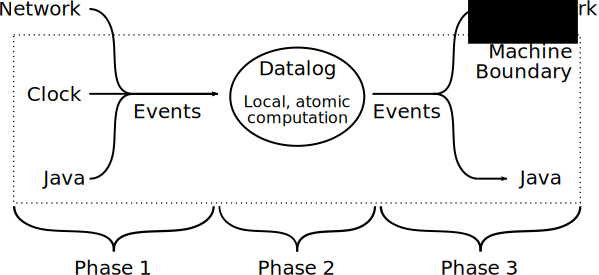
\includegraphics[width=0.95\linewidth]{jol-node.pdf}
    \label{fig:jol-node}
    \caption{An Overlog timestep at a participating node: incoming
      events are applied to local state, the local Datalog program 
      is run to fixpoint, and outgoing events are emitted.}
\vspace{-8pt}
\end{figure}

When Overlog tuples arrive at a node either through rule evaluation or
external events, they are handled in an atomic local Datalog
``timestep.'' Within a timestep, each node sees only locally-stored
tuples.  Communication between Datalog and the rest of the system
(Java code, networks, and clocks) is modeled using \emph{events}
corresponding to insertions or deletions of tuples in Datalog tables.

Each timestep consists of three phases, as shown in Figure~\ref{fig:jol-node}.
In the first phase, inbound events are converted into tuple insertions and
deletions on the local table partitions.  The second phase interprets the local rules and tuples according to traditional Datalog semantics, executing the rules to a ``fixpoint'' in a traditional bottom-up fashion~\cite{ullmanbook},
recursively evaluating the rules until no new results are generated.  In the
third phase, updates to local state are atomically made durable, and outbound
events (network messages, Java callback invocations) are emitted. Note that
while Datalog is defined over a static database, the first and third phases allow
Overlog programs to mutate state over time.

% Communication in Overlog happens as a side-effect of data partitioning. Loo et al.\ show that any Overlog program can be compiled into 
% a form where the body relations join on the same location-specifier variable, so that all relational processing is localized~\cite{loo-sigmod06}.  They also prove eventual consistency of the distributed tables under the rules, when certain simplifying assumptions hold.  In Section~\ref{sec:lessons} we discuss our experience with this model.

%\rcs{Rewrote this; the old discussion doesn't match the current implementation; the difference between the two is important for atomicity + transactions.  OLD: Each timestep consists of five phases.
% , which taken together atomically modify a local database, execute a Datalog program on that database, materialize the consequences of the program, and generate messages.  
%In Phase 1 ({\em Insertion}), inbound tuples are dequeued from a {\em network insertion queue}; each tuple arrives annotated with the name of a table, into which it is inserted\footnote{Tuples that do not conform to the local database schema are inserted into an ``exception'' table that can be configured either to store or drop tuples. \jmh{Is this a lie?}}.  In Phase 2 ({\em Datalog}), the Overlog rules in the system are treated as purely declarative Datalog queries, which are run recursively to their conclusion: a fixpoint where further application of the rules produces no new results. \JOL uses a delta-computation approach to speed up this process~\cite{matview-maintain}. In Phase 3 ({\em Materialization}), the outputs of Phase 2 queries that have the local address in their location specifier are cached in the local database as {\em Materialized Views}~\cite{matview-maintain}; output tuples with remote location specifiers are enqueued to be sent to their appropriate destination.
%Overlog supports syntax for tuple deletion and update as well, as described by Condie~\cite{evitaraced}.  
%  The exception to this processing are the results of Overlog rules prefaced by the {\tt delete} keyword; local {\tt delete} results are enqueued for Phase 4, whereas remote {\tt delete} results are marked as {\tt deletion} tuples before they are enqueued on the network.  \jmh{skipping primary key stuff here; roll in later if needed.} 
%In Phase 4 ({\em Deletion}), tuples are dequeued from an inbound {\em network deletion queue} and combined with the results of deletion tuples derived in Phase 2; taken together, these tuples are processed via deduction to determine any {\em consequent} tuples (previously computed in Phases 2 and 3 at any timestep) that  depend upon them recursively; then the tuples to be deleted {\em and all their local consequents} are deleted from the database; remote deletion consequents are also added to the network queue.  Finally, in Phase 5 ({\em Transmission}) the outbound network queues are flushed using the appropriate network protocols.}

\subsection{JOL}
The original Overlog implementation (\emph{P2}) is aging and targeted at network
protocols, so we developed a new Java-based Overlog runtime we call \emph{\JOL.}
Like P2, \JOL compiles Overlog programs into pipelined dataflow graphs of
operators (similar to ``elements'' in the Click modular router~\cite{click}).
\JOL provides \emph{metaprogramming} support akin to P2's Evita Raced
extension~\cite{evitaraced}: each Overlog program is compiled into a
representation that is captured in rows of tables.  Program testing,
optimization and rewriting can be written concisely as metaprograms in Overlog
that manipulate those tables.

Because the Hadoop stack is implemented in Java, we anticipated the need for
tight integration between Overlog and Java code. Hence, \JOL supports Java-based
extensibility in the model of Postgres~\cite{postgres}.  It supports Java
classes as abstract data types, allowing Java objects to be stored in fields of
tuples, and Java methods to be invoked on those fields from Overlog.  \JOL also
allows Java-based aggregation functions to run on sets of column values, and
supports Java \emph{table functions}: Java iterators producing tuples, which can
be referenced in Overlog rules as ordinary relations. We made significant use of
each of these features in \BOOMA.

  % \rcs{<- too dense; sounds complicated.  replace w/ figure that describes syntax?}  
% Second, \JOL makes use of Java's built-in networking code rather than implementing it as componentized dataflow as in P2.\rcs{<- implementation detail (cut)?}  
% Third, 
%\jmh{Removed discussion of metaprogrammed scheduler since we don't exercise it much.}
%In addition, inspired by the ideas of Evita Raced, we metaprogrammed \JOL's core execution loop and scheduler in Overlog as well.  Rather than using a traditional event loop,  in \JOL all inbound events (i.e., tuples) are passed into a single dataflow compiled from the system's runtime metaprogram. This dataflow ``routes'' tuples to appropriate branches corresponding to different rules, using a scheduler specified in Overlog.  Space prevents a thorough discussion of this design, but we mention it here because of our experience modifying the runtime rules as described in Section~\ref{sec:perf}.  
% \rcs{Fourth, \JOL's design is based upon composition of local datalog processes; P2's execution model attempted to provide coherent datalog semantics across network links.  We believe that \JOL's model leads to more natural handling of issues such as node failure and hetergeneous networks.}

%Our commercial cluster experiments ran on 96 physical nodes spanning 5 racks. Each node has 4 disks, 3 GB of memory, and 8 Intel Xeon processors\rcs{``Intel Xeon'' means nothing... are they 64 bit? Penitum IV generation? Core 2?}, 1.8 GHz each. One node was running the JobTracker, another node was running HDFS's NameNode. The other 94 nodes in the cluster were slaves running both a TaskTracker and a DataNode.

%\jmh{add details ...} \rcs{good enough?}


% \section{Initial Prototype}
% \label{sec:proto}
% Our coding effort began in May, 2008, with an initial implementation
% of \JOL. Development of the Overlog-based version of HDFS (\BOOM-FS)
% started in September of 2008.  We began development of our
% Overlog-based modifications to MapReduce (\BOOM-MR) in January, 2009,
% and the results we report on here are from May, 2009.

% We used two different design styles in developing the two halves of
% \BOOMA.  Our \BOOM-FS implementation began as a clean-slate rewrite in
% Overlog. When we had a prototype file system working in an
% Overlog-only environment, we retrofitted the appropriate Java APIs to
% make it API-compliant with Hadoop.  For \BOOM-MR, by contrast, we
% ported the ``interesting'' material in Hadoop's MapReduce code
% piece-by-piece to Overlog, leaving various API routines in their
% original state in Java.


\section{HDFS Rewrite}
\label{sec:boom-fs}
Our first effort in developing \BOOMA was \BOOM-FS, a clean-slate rewrite of
HDFS in Overlog.  HDFS is loosely based on GFS~\cite{gfs-sosp}, and is targeted
at storing large files for full-scan workloads.  In HDFS, file system metadata
is stored at a centralized \emph{{\NN}}, but file data is partitioned into
\emph{chunks} and distributed across a set of \emph{{\DN}s}. By default, each
chunk is 64MB and is replicated at three {\DN}s to provide fault tolerance. {\DN}s
periodically send heartbeat messages to the {\NN} containing the set of chunks
stored at the {\DN}. The {\NN} caches this information. If the {\NN} has not
seen a heartbeat from a {\DN} for a certain period of time, it assumes that the
{\DN} has crashed and deletes it from the cache; it will also create additional
copies of the chunks stored at the crashed {\DN} to ensure fault tolerance.

Clients only contact the {\NN} to perform metadata operations, such as
obtaining the list of chunks in a file; all data operations involve
only clients and {\DN}s. HDFS only supports file read and append
operations; chunks cannot be modified once they have been written.


%%In contrast to our ``porting'' strategy for implementing \BOOM-MR, we
%%chose to build \BOOM-FS from scratch.  

%%This required us to exercise
%%Overlog more broadly, limiting our Hadoop/Java compatibility task to
%%implementing the HDFS client API in Java.  We did this by creating a
%%simple translation layer between Hadoop API operations and \BOOM-FS
%%protocol commands. The resulting \BOOM-FS implementation works with
%%either vanilla Hadoop MapReduce or \BOOM-MR.

Like GFS, HDFS maintains a clean separation of control and data protocols:
metadata operations, chunk placement and {\DN} liveness are decoupled from the
code that performs bulk data transfers. Following this lead, we implemented the
simple high-bandwidth data path ``by hand'' in Java, concentrating our Overlog
code on the trickier control-path logic. This allowed us to use a prototype
version of \JOL that focused on functionality more than performance. As we
document in Section~\ref{sec:eval}, this was sufficient to allow \BOOM-FS to
keep pace with HDFS in typical MapReduce workloads.

% The Java 
% integration features of \JOL made, we were able to use
% the most appropriate language for the problem at hand. As we reflect
% in Section \ref{sec:lessons}, this produced a hybrid system that is
% both clean and efficient.

\subsection{File System State}
The first step of our rewrite was to represent file system metadata as
a collection of relations (Table~\ref{tab:bfs-schema}). We then
implemented file system operations by writing queries over this
schema.

The \emph{file} relation contains a row for each file or directory stored in
\BOOM-FS\@. The set of chunks in a file is identified by the corresponding rows
in the \emph{fchunk} relation.\footnote{The order of a file's chunks must also
  be specified, because relations are unordered. Currently, we assign chunk IDs
  in a monotonically increasing fashion and only support append operations, so
  clients can determine a file's chunk order by sorting chunk IDs.} The
\emph{datanode} and \emph{hb\_chunk} relations contain the set of live {\DN}s
and the chunks stored by each {\DN}, respectively. The {\NN} updates these
relations as new heartbeats arrive; if the {\NN} does not receive a heartbeat
from a {\DN} within a configurable amount of time, it assumes that the {\DN} has
failed and removes the corresponding rows from these tables.

The {\NN} must ensure that file system metadata is durable and restored to a
consistent state after a failure. This was easy to implement using Overlog; each
Overlog fixpoint brings the system from one consistent state to another. We used
the Stasis storage library~\cite{stasis} to write durable state changes to disk
as an atomic transaction at the end of each fixpoint. Like P2, \JOL allows
durability to be specified on a per-table basis. So the relations in
Table~\ref{tab:bfs-schema} were marked durable, whereas ``scratch tables'' that
are used to compute responses to file system requests were
transient --- emptied at the end of each fixpoint.

\begin{table}
\centering
\scriptsize{
\begin{tabular}{|l|l|l|} \hline
\textit{Name}   & \textit{Description} & \textit{Relevant attributes} \\ \hline\hline
file          & Files   & \underline{fileid}, parentfileid, name, isDir\\ \hline
fqpath & Fully-qualified pathnames & path, \underline{fileid}\\ \hline
fchunk         &  Chunks per file  & \underline{chunkid}, \underline{fileid} \\ \hline
datanode  & {\DN} heartbeats      & \underline{nodeAddr}, lastHeartbeatTime \\  \hline
hb\_chunk  & Chunk heartbeats            & \underline{nodeAddr}, \underline{chunkid},  length\\ \hline
\end{tabular}
}
\caption{\BOOM-FS relations defining file system metadata. The underlined attributes
together make up the primary key of each relation.}
\label{tab:bfs-schema}
\vspace{-8pt}
\end{table}

Since a file system is naturally hierarchical, the ``queries'' needed to
traverse it are recursive. While recursion in SQL is considered somewhat
esoteric, it is a common pattern in Datalog and hence Overlog.  For example, an
attribute of the \emph{file} table describes the parent-child relationship of
files; by computing the transitive closure of this relation, we can infer the
fully-qualified pathname of each file (\emph{fqpath}). The two Overlog rules
that derive \emph{fqpath} from \emph{file} are listed in
Figure~\ref{fig:bfs-path}. Note that when a \emph{file} representing a directory
is removed, all \emph{fqpath} tuples that describe child paths of that directory
are automatically removed (because they can no longer be derived from the
updated contents of \emph{file}).

Because path information is accessed frequently, we configured the \emph{fqpath}
relation to be cached after it is computed. Overlog will automatically update
\emph{fqpath} when \emph{file} is changed, using standard relational view
maintenance logic~\cite{ullmanbook}. \BOOM-FS defines several other views to
compute derived file system metadata, such as the total size of each file and
the contents of each directory. The materialization of each view can be changed
via simple Overlog table definition statements without altering the semantics of
the program. During the development process, we regularly adjusted view
materialization to trade off read performance against write performance and
storage requirements.

At each \DN, chunks are stored as regular files on the file system. In
addition, each {\DN} maintains a relation describing the chunks stored
at that node. This relation is populated by periodically invoking a
table function defined in Java that walks the appropriate directory of
the {\DN}'s local file system.

% \jmh{We reimplemented data nodes, so got to define our own API between them and name nodes}
% For storage of file system data, we had two design choices: leave the HDFS {\DN} implementations as 
% they were and implement the APIs necessary for communication with the new {\NN} and client applications, 
% or replace the {\DN}s as well.  We chose the latter because it was easy to do so: state representation 
% in a {\DN} 
%The state at the {\DN}s is quite simple (a mapping of local chunks to
%sizes and checksums). \jmh{Ref here to details in a schema diagram?}

\subsection{Communication Protocols}
Both HDFS and \BOOM-FS use three different protocols: the \emph{metadata
  protocol} that clients and {\NN}s use to exchange file metadata, the
\emph{heartbeat protocol} that {\DN}s use to notify the {\NN} about chunk
locations and {\DN} liveness, and the \emph{data protocol} that clients and
{\DN}s use to exchange chunks. We implemented the metadata and heartbeat
protocols with a set of distributed Overlog rules.  The data protocol was
implemented in Java because it is simple and performance critical. We proceed to
describe the three protocols in order.

For each command in the metadata protocol, there is a single rule at
the client (stating that a new request tuple should be ``stored'' at
the {\NN}). There are typically two corresponding rules at the {\NN}:
one to specify the result tuple that should be stored at the client,
and another to handle errors by returning a failure message. 
%%An
%%example of the {\NN} rules for Chunk Location requests is shown in
%%Figure~\ref{fig:bfs-chunk-locs}.

Requests that modify metadata follow the same basic structure, except that in
addition to deducing a new result tuple at the client, the {\NN} rules also
deduce changes to the file system metadata relations. Concurrent requests to the
{\NN} are handled in a serial fashion by {\JOL}. While this simple approach has
been sufficient for our experiments, we plan to explore more sophisticated
concurrency control techniques in the future.

\begin{figure}[t]
\centering
\begin{footnotesize}
\begin{verbatim}
// fqpath: Fully-qualified paths.
// Base case: root directory has null parent
fqpath(Path, FileId) :-
    file(FileId, FParentId, _, true),
    FParentId = null, Path = "/";

fqpath(Path, FileId) :-
    file(FileId, FParentId, FName, _),
    fqpath(ParentPath, FParentId),
    // Do not add extra slash if parent is root dir
    PathSep = (ParentPath = "/" ? "" : "/"),
    Path = ParentPath + PathSep + FName;
\end{verbatim}
\end{footnotesize}
\vspace{-8pt}
\caption{Example Overlog for deriving fully-qualified pathnames from
  the base file system metadata in \BOOM-FS.}
\label{fig:bfs-path}
\vspace{-8pt}
\end{figure}


%%\begin{figure}
%%\centering
%%\begin{footnotesize}
%%\begin{verbatim}
%%// The set of nodes holding each chunk
%%compute_chunk_locs(ChunkId, set<NodeAddr>) :-
%%    hb_chunk(NodeAddr, ChunkId, _);

%%// Chunk exists => return success and set of nodes
%%response(@Src, RequestId, true, NodeSet) :-
%%    request(@Master, RequestId, Src,
 %%           "ChunkLocations", ChunkId),
%%    compute_chunk_locs(ChunkId, NodeSet);

%%// Chunk does not exist => return failure
%%response(@Src, RequestId, false, null) :-
%%    request(@Master, RequestId, Src,
%%            "ChunkLocations", ChunkId),
%%    notin hb_chunk(_, ChunkId, _);
%%\end{verbatim}
%%\end{footnotesize}
%%\vspace{-12pt}
%%\caption{{\NN} rules to return the set of {\DN}s that hold a given
%%  chunk in \BOOM-FS.}
%%\label{fig:bfs-chunk-locs}
%%\vspace{-2pt}
%%\end{figure}

The heartbeat protocol follows a similar request/response pattern, but it is not
driven by the arrival of network events. In order to trigger such events in a
data-centric language, Overlog offers a \emph{periodic} relation~\cite{p2} that
can be configured to produce new tuples at every tick of a wall-clock
timer. {\DN}s use the \emph{periodic} relation to send heartbeat messages to
{\NN}s.

The {\NN} can also send control messages to {\DN}s. This occurs when a file
system invariant is unmet and the {\NN} requires the cooperation of the {\DN} to
restore the invariant. For example, the {\NN} records the number of replicas of
each chunk (as reported by heartbeat messages). If the number of replicas of a
chunk drops below the configured replication factor (e.g., due to a {\DN}
failure), the {\NN} sends a message to a {\DN} that stores the chunk, asking it
to send a copy of the chunk to another {\DN}.

Finally, the data protocol is a straightforward mechanism for
transferring the contents of a chunk between clients and {\DN}s. This
protocol is orchestrated by Overlog rules but implemented in
Java. When an Overlog rule deduces that a chunk must be transferred
from host \emph{X} to \emph{Y}, an output event is triggered at
\emph{X}. A Java event handler at \emph{X} listens for these output
events and uses a simple but efficient data transfer protocol to send
the chunk to host \emph{Y}. To implement this protocol, we wrote a
simple multi-threaded server in Java that runs on the {\DN}s.

\begin{table}
\centering
\scriptsize{
\begin{tabular}{|l|r|r|} \hline
\textit{System}   & \textit{Lines of Java} & \textit{Lines of Overlog} \\ \hline\hline
HDFS       & \texttildelow{}21,700   & 0 \\ \hline
\BOOM-FS & 1,431    & 469 \\ \hline
\end{tabular}
}
\caption{Code size of two file system implementations.}
\label{tbl:boomfs}
\vspace{-8pt}
\end{table}

\subsection{Discussion}
\label{sec:hdfs-discuss}
After four person-months of work, we had a working implementation of metadata
handling in Overlog, and it was straightforward to add Java code to store chunks
in UNIX files. Adding metadata durability took about a day.  Adding the
necessary Hadoop client APIs in Java took an additional week.  As
Table~\ref{tbl:boomfs} shows, \BOOM-FS contains an order of magnitude less code
than HDFS\@. The \DN implementation accounts for 414 lines of the Java in
\BOOM-FS; the remainder is devoted to system configuration, bootstrapping, and a
client library. Adding support for accessing \BOOM-FS via Hadoop's API required
an additional 400 lines of Java.

In retrospect, the main benefit of our data-centric approach was to expose the
simplicity of HDFS's core state, which consists of simple file system metadata
and streams of messages in a few communication protocols.  Having identified the
relevant data and captured it in relations, the task of writing code to
coordinate the data was relatively easy and could have been written fairly
quickly in any language with good support for collection types.

Beyond this data-centric approach, the clearest benefit of Overlog's
declarativity at this stage turned out to be the ability to (a) express paths as
simple recursive queries over parent links, and (b) flexibly decide when to
maintain materialized views (i.e., cached or precomputed results) of those paths
separate from their specification.\footnote{In future, these decisions could be
  suggested or made automatic by an optimizer based on data and workloads.}
Overlog's built-in support for persistence, messaging, and timers were also
convenient, and enabled file system policy to be stated concisely.

When we began this work, we expected that using a declarative language would
allow the natural specification and maintenance of file system invariants. We
found that this was only partially true. For {\NN}-local invariants (e.g.,
ensuring that the \emph{fqpath} relation is consistent with the \emph{file}
relation), Overlog gave us confidence in the correctness of our system. However,
Overlog was less useful for describing invariants that require the coordination
of multiple nodes (e.g., ensuring that the replication factor of each chunk is
satisfied). On reflection, this is because distributed Overlog rules induce
asynchrony across nodes; hence, such rules must describe \emph{protocols} to
enforce distributed invariants, not the invariants themselves. Hence, the code
we wrote to maintain the replication factor of each chunk had a low-level,
``state machine''-like flavor. We return to this point in
Section~\ref{sec:overlog-lessons}.

Although \BOOM-FS replicates the basic architecture and functionality of HDFS,
we did not attempt to achieve feature parity.  HDFS features that \BOOM-FS does
not support include file access permissions, a web interface for status
monitoring, and proactive rebalancing of chunks among {\DN}s in a cluster. Like
HDFS, the initial \BOOM-FS prototype avoids distributed systems and parallelism
challenges by implementing coordination with a single centralized \NN.  It can
tolerate \DN failures but has a single point of failure and scalability
bottleneck at the \NN. We discuss how we improved \NN fault tolerance and
scalability in Sections~\ref{sec:rely} and \ref{sec:scale}, respectively. As we
discuss in Section~\ref{sec:eval}, the performance of \BOOM-FS is competitive
with HDFS\@.


% In Hadoop 18, each map or reduce task is executed in a newly-spawned
% child process. In our initial \BOOM-FS prototype, each process created
% a new copy of the JOL interpreter. This resulted in poor performance,
% because the current version of JOL takes \textasciitilde{}1.5 seconds
% to create an instance of the interpreter, which can be a significant
% portion of the total runtime of a typical map task. To avoid this
% problem, we modified Hadoop to spawn a single ``JOL server'' process
% at each worker node. To access \BOOM-FS, map and reduce tasks
% communicate with the JOL server process using RPCs. This issue could
% also have been mitigated by using the ``reuse JVMs'' capability
% introduced in Hadoop 19.

% , and we feel
% that \BOOM-FS reflects that simplicity well.  HDFS sidesteps many of
% the performance challenges of traditional file systems and databases
% by focusing nearly exclusively on scanning large files.  It  As a result, most of our implementation consists of simple
% message handling and management of the hierarchical file system
% namespace. Datalog materialized view logic was not hard to implement
% in \JOL, and took care of most of the performance issues we faced over
% the course of our development.



\section{The Availability Rev}
\label{sec:rely}
% \paa{a basic substrate for a HA distributed system is a total ordering over events; cf Lamport's state machine
% approach.  this amounts to a distributed log.  Paxos is commonly used to achieve this property.
% the harvard guys showed that a logic language Paxos was possible, but did not produce a useable implementation 
% (single-decree basicPaxos, races, etc).  we needed to make it "live" and encountered many of the issues
% mentioned by the chubby authors, which are NOT treated (other than being mentioned) in the lamport literature.
% discuss the "glue" needed to Paxos-ize bfs.  putting state changes into the Paxos log is the easy part: stringify.
% trickier is crafting the rules that are contingent on reading an entry from the log; ie, user sends a "create file"
% request, we pass it through Paxos.  deltas on the "passed decrees" log trigger rules that reflect the new file in
% the current metadata, and send the response to the client.
% discussion of how reliability is tested..
% }


% In a single-node system, reliability is directly tied to recoverability, and is typically guaranteed by a 
% combination of redundant storage (i.e. RAID) and logging (i.e. WAL logs in databases and journals in file 
% systems).  

% \jmh{I have added para-by-para annotations here to see if we like the flow, and help us think about condensing/refocusing.}
% 
% \jmh{The shtick: Base implementation done, it was time for a feat of
% distributed derring-do.}
Having achieved a fairly faithful implementation of HDFS, we were ready to
explore whether data-centric programming would make it easy to add complex
distributed functionality to an existing system.  We chose what we considered a
challenging goal: retrofitting \BOOM-FS with high availability failover via
``hot standby'' {\NN}s.  A proposal for warm standby was posted to the Hadoop
issue tracker in October of 2008 (\cite{jira} issue HADOOP-4539). We felt that a
hot standby scheme would be more useful, and would more aggressively test our
hypothesis that significant distributed system infrastructure could be
implemented cleanly in a data-centric manner.

%\jmh{Background -- real heroes do it via Paxos.}
\subsection{Paxos Implementation}
Implementing hot standby replication is tricky, since replica state must remain
consistent in the face of node failures and lost messages. One solution is to
use a globally-consistent distributed log, which guarantees a total ordering
over events affecting replicated state. Lamport's Paxos algorithm is the
canonical mechanism for this feature~\cite{part-time}.

%\jmh{What were we thinking?  This para may be unnecessarily long.}
% We had two reasons to believe that we could cleanly retrofit a hot
% standby solution into \BOOM-FS.  First, data-centric programming had
% already forced us to encode the relevant \NN state into a small number
% of relational tables, so we knew what data we needed to
% replicate. Second, we were encouraged by a concise Overlog
% implementation of simple Paxos that had been achieved in an early
% version of P2~\cite{paxonp2}.  On the other hand, we were sobered by
% the fact that the Paxos-in-P2 effort failed to produce a useable
% implementation; like the Paxos implementation at
% Google~\cite{paxos-live}, they discovered that Lamport's
% papers~\cite{paxos-simple, part-time} present just a sketch of what
% would be necessary to implement Paxos in a practical environment.
% last clause of this paragraph can be removed, I think ~nrc

% \jmh{First step: simple Paxos validates data-centric language.}
We began by creating an Overlog implementation of basic Paxos, focusing on
correctness and adhering as closely as possible to the initial
specification. Lamport's description of Paxos is given in terms of ``ballots''
and ``ledgers,'' which correspond to network messages and stable storage,
respectively. The consensus algorithm is given as a collection of logical
invariants which describe when agents cast ballots and commit writes to
their ledgers.  In Overlog, messages and disk writes are represented as
insertions into tables with different persistence properties, while invariants
are expressed as Overlog rules.  Our first effort was clean and fairly simple:
22 Overlog rules in 53 lines of code, corresponding nearly line-for-line with
the invariants from Lamport's original paper~\cite{part-time}.  Since our entire
implementation fit on a single screen, we were able to visually confirm its
faithfulness to the original specification.  To this point, working with a
data-centric language was extremely gratifying, as we further describe
in~\cite{netdb-declare}.

%\jmh{Now, get real.  Not quite as pretty.}
Next, we needed to convert basic Paxos into a working primitive for a
distributed log.  This required adding the ability to efficiently pass a series of log
entries (``Multi-Paxos''), a liveness module, and a catchup algorithm. While the
first was for the most part a simple schema change, the latter two caused our
implementation to swell to 50 rules in roughly 400 lines of code. Echoing the experience of
Chandra et al.~\cite{paxos-live}, these enhancements made our code considerably
more difficult to check for correctness. The code also lost some of its pristine
declarative character; we return to this point in Section~\ref{sec:lessons}.

%%This was due in part to the evolution of the Paxos research
%%papers: while the original Paxos was described as a set of invariants
%%over state \jmh{say this in previous paragraph!}, most of the optimizations were described as transition
%%rules in state machines.
%\jmh{Is there a pithy example of this?} 
%%Hence we found ourselves translating state-machine pseudocode back into logical invariants, and it took some time to gain confidence in our code.  The resulting 
%%implementation is still very concise relative to a traditional programming language, but it highlighted the difficulty of using a data-centric programming model for 
%%complex tasks that were not originally specified that way. \jmh{Is this about data-centric or about logic?} 

\subsection{\BOOM-FS Integration}
\label{sec:paxos-integration}
%\jmh{Integration is simple, though.}
Once we had Paxos in place, it was straightforward to support the replication of
file system metadata. All state-altering actions are represented in the revised
\BOOM-FS as Paxos decrees, which are passed into the Paxos logic via a single
Overlog rule that intercepts tentative actions and places them into a table that
is joined with Paxos rules. Each action is considered complete at a given site
when it is ``read back'' from the Paxos log (i.e., when it becomes visible in a
join with a table representing the local copy of that log). A sequence number
field in the Paxos log table captures the globally-accepted order of actions on
all replicas.

%%\nrc{Kill this paragraph, or move to previous section.}
%%We also had to ensure that Paxos state was durable in the face of crashes.
%%Lamport's description of Paxos explicitly distinguishes between transient and
%%durable state. Our implementation already divided this state into separate
%%relations, so we simply marked the appropriate relations as durable.

%\jmh{
% hard to read!
% For atomic, unconditional actions, the Paxos layer merely chooses a serialization order. In the more common case, however, a submitted action must be validated against the current application state.  In this case, an action is accepted by a replica only if it represents a transition to a new consistent state.  Because Paxos guarantees that all replicas see the same set of transitions in the same order, if a tentative action is refused on one replica it will be refused everywhere.  A series of actions that must be treated as an atomic unit may be converted into a``multi-op'' \cite{paxos-live}
% our Paxos rules made use of a guard clause and a set of actions to be executed upon the success or failure of the guard. <-- huh?  I don't really understand.} \rcs{multi-op?  what's that?  is this something we do?  Also, the stasis description means it no longer fits here.} 
% \paa{
%     we can omit the preceeding.  that paxos enforces an order, and that all replicas make the same set of transitions, is the whole point of using a consensus protocol.  the paxos made live authors discuss the usefulness of the multi-op primitive; we don't use it in bfs so there's no point discussing it here.
% }
% Finally, to implement Paxos we had to ensure that the appropriate
% tables were stored persistently, and restored to consistency after a
% failure. As for \BOOM-FS itself, we used the 
% Finally, to implement Paxos reliably we had to add a disk persistence mechanism to \JOL, a feature that was not considered in P2.  We chose to use the Stasis storage library~\cite{stasis}, which provides atomicity and durability for concurrent transactions, and handles physical consistency of its indexes and other internal structures. 
% Unlike many transactional storage libraries, Stasis does not provide a default mechanism for concurrency control.  This suited our purposes well, since Overlog's timestep semantics isolate the local database from network events, and take it from one consistent fixpoint to another.
 % However, it does not provide consistency or isolation over ``application'' state, such as the tuples stored in \JOL's tables.  By leaving concurrency control to client code, Stasis is able to make use of deadlock avoidance instead of deadlock detection, and will never force \JOL to roll-back transactions at runtime.  Since \JOL does not contain a notion of transactional abort, recovering from storage deadlocks would have complicated our design considerably.  For Stasis recovery to work correctly, \JOL must still ensure ``Consistency'' and ``Isolation'' for its ACID transactions.  By definition, Datalog fixpoints transform application data from one consistent state to another.  Also, \JOL queues up incoming and outgoing network messages during fixpoint computation, providing isolation.  Therefore, 
% We implemented each \JOL fixpoint as a single Stasis transaction.  

% \paa{ I don't agree with the point about isolation.  when I think of isolation I think of database-transaction-style solipsism: I can write a program that pretends it isn't possible that my execution could be interleaved with that of another program.  I don't believe that this is true in overlog: the programmer needs to reason about concurrency because fixpoints process batches of tuples from potentially many other nodes, and the order and timing of these events can be arbitrary.  
% }

% Many of the tables in \BOOMA represent transient in-memory data
% structures, even though they are represented as ``database'' tables.
% Hence we decided to allow \JOL programs to decide which tables should
% be durably stored in Stasis, and which should be transient.  Fixpoints
% that do not touch durable tables do not create Stasis transactions.

We validated the performance of our implementation experimentally. In the
absence of failure, replication has negligible performance impact, but when the
primary \NN fails, a backup \NN takes over reasonably quickly.  We present
performance results in the technical report~\cite{boom-techr}.

% Rusty notes:
% \begin{itemize}
% \item
%   RCS Local durability primitive: Force persistent tables at end of
%   timestamp.  (Paxos 'just works' (?)) Need datalog rewrite for 2PC's
%   prepare (ie: transactions in datalog rewrites).  2PC would be a
%   forward ref to performance section if it is here.  Splitting 2PC
%   into perf section might confuse durability story.
% 
% \item
%   Replicated HDFS master nodes ($\to$ crash recovery; assuming we have
%   enough elements in the log?)
% 
% \end{itemize}

\subsection{Discussion}
Our Paxos implementation constituted roughly 400 lines of code and required six
person-weeks of development time. Adding Paxos support to \BOOM-FS took two
person-days and required making mechanical changes to ten \BOOM-FS rules (as
described in Section~\ref{sec:paxos-integration}). We suspect that the rule
modifications required to add Paxos support could be performed as an automatic
rewrite.

% \jmh{I need help here separating out the benefits of reifying data from using
% Overlog.  However we do it we need to tone down the self-praise.  This subsection needs work.}
% The Availability revision was our first foray into ``serious''
% distributed systems programming, and we continued to benefit from the
% high-level abstractions provided by Overlog.  Most of our attention
% was focused at the appropriate level of complexity: faithfully
% capturing the reasoning involved in distributed protocols.
% \paa{not sure what to do with the previous sentence}

Lamport's original paper describes Paxos as a set of logical invariants.  This
specification naturally lent itself to a data-centric design in which
``ballots,'' ``ledgers,'' internal counters and vote-counting logic are
represented uniformly as tables.  However, as we note in a workshop
paper~\cite{netdb-declare}, the principal benefit of our approach came directly
from our use of a rule-based declarative language to encode Lamport's
invariants.  We found that we were able to capture the design patterns
frequently encountered in consensus protocols (e.g., multicast, voting) via the
composition of language constructs like aggregation, selection and join.

In our initial implementation of basic Paxos, we found that each rule covered a
large portion of the state space, avoiding the case-by-case transitions that
would need to be specified in a state machine-based implementation.  However,
choosing an invariant-based approach made it harder to adopt optimizations from
the literature as the code evolved, in part because these optimizations were
often described using state machines. We had to choose between translating the
optimizations ``up'' to a higher-level while preserving their intent, or
directly ``encoding'' the state machine into logic, resulting in a
lower-level implementation.  In the end, we adopted both approaches, giving
sections of the code a hybrid feel.

%%For example, a common optimization of basic Paxos avoids
%%the high messaging cost of reaching quorum by skipping the protocol's
%%first phase once a master has established quorum: subsequent decrees
%%then use the established quorum, and merely hold rounds of voting
%%while steady state is maintained.  This is naturally expressed in a
%%state machine model as a pair of transition rules for the same input
%%(a request) given different starting states.  
%%In our implementation,
%%we frequently found it easier in such cases to model the state as a relation
%%with a single row, allow certain rules to fire only in certain 
%%states, and explicitly describe the transitions, rather than to reformulate
%%the optimizations in terms of original logic.  Though mimicking a state 
%%machine is straightforward, the resulting rules have a 
%%hybrid feel, which somewhat compromises our high-level protocol specification.

% These are simple uses of Overlog
% persistence, but for our purposes to date this model has been
% sufficient.  Stasis was an elegant fit due to its separation of
% atomic, durable writes from traditional transactional locking for
% isolation and consistency.  However, given the modest load we put on
% Stasis, we also would probably have been fine using a traditional
% database.

%\jmh{We return to this point in Section~\ref{sec:lessons}.}


\section{The Scalability Rev}
\label{sec:scale}
% \begin{itemize}
% \item
%   Partitioned HDFS master node (done)
% \item
%   Debugging at scale (tyson's tracker load view vs. scheduler load view).
% \item
%   There must be more things...
% \end{itemize}

HDFS {\NN}s manage large amounts of file system metadata, which are kept in
memory to ensure good performance. The original GFS paper acknowledged that this
could cause significant memory pressure~\cite{gfs-sosp}, and \NN scaling is
often an issue in practice at Yahoo!.  Given the data-centric nature of
\BOOM-FS, we hoped to simply scale out the \NN across multiple
\emph{\NN-partitions}. Having exposed the system state in tables, this was
straightforward: it involved adding a ``partition'' column to various tables to
split them across nodes in a simple way. Once this was done, the code to query
those partitions --- regardless of language in which it is written --- composes
cleanly with our availability implementation: each \NN-partition can be deployed
either as a single node or a Paxos group.

There are many options for partitioning the files in a directory tree.  We opted
for a simple strategy based on the hash of the fully-qualified pathname of each
file.  We also modified the client library to broadcast requests for directory
listings and directory creation to every \NN-partition.  Although the resulting
directory creation implementation is not atomic, it is idempotent; recreating a
partially-created directory will restore the system to a consistent state, and
will preserve any files in the partially-created directory. For all other
\BOOM-FS operations, clients have enough local information to determine the
correct \NN-partition. 

We did not attempt to support atomic ``rename'' across partitions. This would
involve the atomic transfer of state between independent Paxos groups.
We believe this would be relatively straightforward to implement --- we have
previously built a two-phase commit protocol in Overlog~\cite{netdb-declare} ---
but we decided not to pursue this feature at present.

%\jmh{Figure~\ref{fig:scaling} shows...}

\subsection{Discussion}
By isolating the file system state into relations, it became a textbook exercise
to partition that state across nodes.  It took eight hours of developer time to
implement \NN partitioning; two of these hours were spent adding partitioning
and broadcast support to the \BOOM-FS client library.  This was a clear win for
the data-centric approach, independent of any declarative features of Overlog.

Before attempting this work, we were unsure whether partitioning for scale-out
would compose naturally with state replication for fault tolerance. Because
scale-out in \BOOM-FS amounted to little more than partitioning data
collections, we found it quite easy to convince ourselves that our scalability
improvements integrated correctly with Paxos. Again, this was primarily due to
the data-centric nature of our design. Using a declarative language
led to a concise codebase that was easier to understand, but the essential
benefits of our approach would likely have applied to a data-centric
implementation in a traditional imperative language.


\section{The Monitoring Rev}
\label{sec:manage}
As our \BOOMA prototype matured and we began to refine it, we started to suffer
from a lack of performance monitoring and debugging tools. As Singh et al.\
observed, Overlog is in essence a stream query language, well-suited to writing
distributed monitoring queries~\cite{singh-eurosys}.  This offers a naturally
introspective approach: simple Overlog queries can monitor complex protocols.
Following that idea, we decided to develop a suite of debugging and monitoring
tools for our own use in Overlog.

%\jmh{Our first effort on this front was to simply annotate our code with logical constraints.  Is this stuff just coding discipline, or did we introduce some kind of language feature here?  And what is all this discussion of ``outermost enclosing Overlog programs''?}

%\paa{we introduced the trivial language feature of the distinguished predicate ("die") that will create an exception in the host language via a callback.  similar to what boon describes in the lbtrust work}

\subsection{Invariants}
\label{sec:invar}
%\jmh{I'm still not too happy with this subsection.  I asked Brewer and Remzi for more cites on the ``maxim'', and if they can't suggest anything we should reword less pedantically.}
One advantage of a logic-oriented language like Overlog is that system
invariants can easily be written declaratively and enforced by the runtime.
This includes ``watchdog rules'' that provide runtime checks of program behavior.
 % --- in fact, local rules in Overlog are essentially invariant specifications over derived relations.  It is often useful to add additional ``watchdog'' invariants to debug an Overlog program, even though they are not required during execution.  
For example, a simple watchdog rule can check that the number of messages sent by a
protocol like Paxos matches the specification.  
%\jmh{Idea for future work: static inference of such properties from rulesets (perhaps a formal execution model required?)  Start with this precise example!}
% Formally, this may be implicit in the protocol specification, and hence redundant.  But the redundancy only holds if the protocol is correctly specified; the point of adding such logic is to ensure that the specification is correct.   Moreover, 
% \nrc{Is the following text relevant? Interesting, probably true, but why do I care?} Distributed Overlog rules induce asynchrony across nodes; such rules are only {\em attempts} to achieve invariants.  An Overlog program needs to be enhanced with global coordination mechanisms like two-phase commit or distributed snapshots to convert distributed Overlog rules into global invariants~\cite{chandylamport}.  Singh et al.\ have shown how to implement Chandy-Lamport distributed snapshots in Overlog~\cite{singh-eurosys}; we did not go that far in our own implementation.  

To simplify debugging, we wanted a mechanism to integrate Overlog invariant
checks into Java exception handling.  To this end, we added a relation called
\emph{die} to \JOL; when tuples are inserted into the \emph{die} relation, a Java
event listener is triggered that throws an exception.  This feature makes it
easy to link invariant assertions in Overlog to Java exceptions: one writes an
Overlog rule with an invariant check in the body, and the \emph{die} relation in
the head. Our use of the \emph{die} relation is similar to the \emph{panic}
relation described by Gupta et al.~\cite{panic}.

% \jmh{This is an example of a ``listener'' that we mentioned earlier; we need a name for update-oriented table functions.}


We made extensive use of these local-node invariants in our code and unit tests.
Although these watchdog rules increase the size of a program, they improve both
reliability and readability.  In fact, had we been coding in Java rather than
Overlog we would likely have put the same invariants in natural language
comments, and ``compiled them'' into executable form via hand-written routines
below the comments (with the attendant risk that the Java does not in fact
achieve the semantics of the comment).  We found that adding invariants of this
form was especially useful given the nature of Overlog: the terse syntax means
that program complexity grows rapidly with code size.  Assertions that we
specified early in the implementation of Paxos aided our confidence in its
correctness as we added features and optimizations.

\subsection{Monitoring via Metaprogramming}
\label{sec:monitor}
Our initial prototype of \BOOM-FS had significant performance problems.
Unfortunately, Java-level performance tools were of little help. A poorly-tuned
Overlog program spends most of its time in the same routines as a well-tuned
Overlog program: in dataflow operators like Join and Aggregation.  Java-level
profiling lacks the semantics to determine which Overlog rules are causing the
lion's share of the runtime.

It is easy to do this kind of bookkeeping directly in
Overlog.  In the simplest approach, one can replicate the body of each
rule in an Overlog program and send its output to a log table (which
can be either local or remote). For example, the Paxos rule that tests
whether a particular round of voting has reached quorum:

{\footnotesize
\begin{verbatim}
  quorum(@Master, Round) :-
      priestCnt(@Master, Pcnt),
      lastPromiseCnt(@Master, Round, Vcnt),
      Vcnt > (Pcnt / 2);
\end{verbatim}
}
\noindent
might have an associated tracing rule:
{\footnotesize
\begin{verbatim}
  trace_r1(@Master, Round, RuleHead, Tstamp) :-
      priestCnt(@Master, Pcnt),
      lastPromiseCnt(@Master, Round, Vcnt),
      Vcnt > (Pcnt / 2),
      RuleHead = "quorum",
      Tstamp = System.currentTimeMillis();
\end{verbatim}
}
\noindent
This approach captures per-rule dataflow in a trace relation that can
be queried later.  Finer levels of detail can be achieved by
``tapping'' each of the predicates in the rule body separately in a
similar fashion.  The resulting program passes no more than twice as
much data through the system, with one copy of the data being ``teed
off'' for tracing along the way.  When profiling, this overhead is
often acceptable. However, writing the trace rules by hand is tedious.

Using the metaprogramming approach of Evita Raced~\cite{evitaraced},
we were able to automate this task via a \emph{trace rewriting} program
written in Overlog, involving the meta-tables of rules and terms.  The
trace rewriting expresses logically that for selected rules of some
program, new rules should be added to the program containing the body
terms of the original rule and auto-generated head terms. Network
traces fall out of this approach naturally: any dataflow transition
that results in network communication is flagged in the generated head
predicate during trace rewriting.

% For example, a rule like:
% {\small
% \begin{verbatim}
% sendPrepare(@Peer,Round,Decree,Agent) :-
%   prepare(@Agent,Round,Decree),
%   Round >= 0, parliament(@Agent,Peer);
% \end{verbatim}
% }
% \noindent
% specifies that each tuple of \texttt{\small prepare} with Round > 0 should be joined with each tuple of \texttt{\small prepare}, and the resulting projected tuple should be sent to the location in its second field and stored in table \texttt{\small sendPrepare}.  This rule can cause the addition of a network trace rule:
% {\small 
% \begin{verbatim}
% tap_out_sendPrepare(Peer,Round,Decree,@Agent) :-
%   prepare(@Agent,Round,Decree),
%   Round >= 0, parliament(@Agent,Peer);
% \end{verbatim}
% }
% \noindent
% that logs the message to be sent; it can also cause the addition of a rule:
% {\small 
% \begin{verbatim}
% tap_in_sendPrepare(@Peer,Round,Decree,Agent) :-
%   prepare(@Agent,Round,Decree),
%   Round >= 0, parliament(@Agent,Peer);
% \end{verbatim}
% }
% \noindent
% that logs the messages received.  Note the difference in the location specifiers (\at) in the two head relations.

Using this idea, it took less than a day to create a general-purpose Overlog
code coverage tool that traced the execution of our unit tests and reported
statistics on the ``firings'' of rules in the \JOL runtime, and the counts of
tuples deduced into tables. We ran our regression tests through this tool, and
immediately found both ``dead code'' rules in our programs, and code that we
knew needed to be exercised by the tests but was as-yet uncovered.

\subsection{Discussion}
The invariant assertions described in Section~\ref{sec:invar} are expressed in
12 Overlog rules (60 lines of code).  We added assertions incrementally over the
lifetime of the project; while a bit harder to measure than our more focused
efforts, we estimate this at no more than 8 person-hours in total.  The
monitoring rewrites described in Section~\ref{sec:monitor} required 15 rules in
64 lines of Overlog. We also wrote a tool to present the trace summary to the
end user, which constituted 280 lines of Java. Because \JOL already provided the
metaprogramming features we needed, it took less than one developer day to
implement these rewrites.

Capturing parser state in tables had several benefits.  Because the program code
itself is represented as data, introspection is a query over the metadata catalog,
while automatic program rewrites are updates to the catalog tables.  Setting up
traces to report upon distributed executions was a simple matter of writing
rules that query existing rules and insert new ones.

Using a declarative, rule-based language allowed us to express assertions in a
``cross-cutting'' fashion.  A watchdog rule describes a query over system state
that must never hold: such a rule is both a specification of an invariant and a
check that enforces it.  The assertion need not be closely coupled with the
rules that modify the relevant state; instead, assertion rules may be written as
a independent collection of concerns.


\section{MapReduce Port}
\label{sec:mr}
In contrast to our clean-slate strategy for developing \BOOM-FS, we built
\BOOM-MR, our MapReduce implementation, by replacing Hadoop's core scheduling
logic with Overlog. Our goal in building \BOOM-MR was to explore embedding a
data-centric rewrite of a non-trivial component into an existing procedural
system.  MapReduce scheduling policies are one issue that has been treated in
recent literature (e.g.,~\cite{late-sched,delay-sched}).  To enable credible
work on MapReduce scheduling, we wanted to remain true to the basic structure of
the Hadoop MapReduce codebase, so we proceeded by understanding that code,
mapping its core state into a relational representation, and then writing
Overlog rules to manage that state in the face of new messages delivered by the
existing Java APIs.  We follow that structure in our discussion.

\subsection{Background: Hadoop MapReduce}
In Hadoop MapReduce, there is a single master node called the \emph{\JT} which
manages a number of worker nodes called \emph{{\TT}s}.  A job is divided into a
set of map and reduce \emph{tasks}. The {\JT} assigns tasks to worker nodes.  Each
map task reads an input chunk from the distributed file system, runs a
user-defined map function, and partitions output key/value pairs into hash
buckets on the local disk.  Reduce tasks are created for each hash
bucket.  Each reduce task fetches the corresponding hash buckets from all
mappers, sorts locally by key, runs a user-defined reduce function and writes
the results to the distributed file system.

Each {\TT} has a fixed number of slots for executing tasks (two maps and two
reduces by default). A heartbeat protocol between each {\TT} and the {\JT} is
used to update the {\JT}'s bookkeeping of the state of running tasks, and drive
the scheduling of new tasks: if the {\JT} identifies free {\TT} slots, it will
schedule further tasks on the {\TT}. Also, Hadoop will attempt to schedule
\emph{speculative} tasks to reduce a job's response time if it detects
``straggler'' nodes~\cite{mapreduce-osdi}.

\subsection{MapReduce Scheduling in Overlog}
\label{sec:mr-overlog}
Our initial goal was to port the {\JT} code to Overlog.  We began by identifying
the key state maintained by the {\JT}.  This state includes both data structures
to track the ongoing status of the system and transient state in the form of
messages sent and received by the {\JT}.  We captured this information in four
Overlog tables, shown in Table~\ref{tbl:hcatalog}.

\begin{table}
\centering
\scriptsize{
\begin{tabular}{|l|l|l|} \hline
\textit{Name}   & \textit{Description} & \textit{Relevant attributes} \\ \hline\hline
job          & Job definitions   & \underline{jobid}, priority, submit\_time, \\ 
             &                   & status, jobConf \\ \hline
task         & Task definitions  & \underline{jobid}, \underline{taskid}, type, partition, status \\ \hline
taskAttempt  & Task attempts      & \underline{jobid}, \underline{taskid}, \underline{attemptid}, progress, \\
             &       & state, phase, tracker, input\_loc, \\ 
             &       & start, finish \\ \hline
taskTracker  & {\TT}             & \underline{name}, hostname, state, \\
             & definitions       & map\_count, reduce\_count, \\
             &                   & max\_map, max\_reduce\\ \hline
\end{tabular}
}
\caption{\BOOM-MR relations defining {\JT} state.}
\vspace{-8pt}
\label{tbl:hcatalog}
\end{table}

The \emph{job} relation contains a single row for each job submitted to the
{\JT}. In addition to some basic metadata, each job tuple contains an attribute
called \emph{jobConf} that holds a Java object constructed by legacy Hadoop
code, which captures the configuration of the job. The \emph{task} relation
identifies each task within a job. The attributes of this relation identify the
task type (map or reduce), the input ``partition'' (a chunk for map tasks, a
bucket for reduce tasks), and the current running status.

A task may be attempted more than once, due to speculation or if the initial
execution attempt failed.  The \emph{taskAttempt} relation maintains the state
of each such attempt.  In addition to a progress percentage and a state
(running/completed), reduce tasks can be in any of three phases: copy, sort, or
reduce. The \emph{tracker} attribute identifies the {\TT} that is assigned to
execute the task attempt. Map tasks also need to record the location of their
input data, which is given by \emph{input\_loc}. The \emph{taskTracker} relation
identifies each {\TT} in the cluster with a unique name.

%It is also used to constrain the scheduler, which can assign map and reduce tasks up to the max\_map and max\_reduce attributes of each tracker. %\jmh{drop dirty?}
%The hostname, current running state, and task workload of the \TT are also part of this relation. 
%The map\_count and reduce\_count attributes indicate how many map and reduce tasks are currently running on the \TT. The maximum number of map and reduce tasks that the \TT is able to support are given by the max\_map and max\_reduce attributes; this is in keeping with Hadoop which specifies these values in each message from a \TT to the \JT.

%Having ``table-ized'' the \JT internals, we still had to translate from the traditional Java-based Hadoop APIs into this representation.  For inbound messages, we stubbed out the original Java message handlers to place tuples on the \JOL event queue, where they are picked up by the \JOL runtime. We chose to leave Hadoop's job configuration parsing untouched; it populates the jobConf field of the {\em job} table. We wrote our Overlog rules to place outbound messages into the {\em trackerAction} table of Table~\ref{tbl:hcatalog}.  We then modified Hadoop's Java heartbeat code to drain this table via a simple \JOL call between timesteps, and send the corresponding API action to the \TT mentioned in each {\em trackerAction} tuple.  \jmh{Isn't this out-of-date?  I.e. we don't invoke Hadoop API calls to talk to the TaskTracker anymore.}


Overlog rules are used to update the {\JT}'s tables by converting inbound messages
into \emph{job}, \emph{taskAttempt} and \emph{taskTracker} tuples. These rules
are mostly straightforward. Scheduling decisions are encoded in the
\emph{taskAttempt} table, which assigns tasks to {\TT}s. A scheduling policy is
simply a set of rules that join against the \emph{taskTracker} relation to find
\TT{}s with unassigned slots, and schedules tasks by inserting tuples into
\emph{taskAttempt}. This architecture makes it easy for new scheduling policies
to be defined.

%%\begin{table}[h]
%%\centering
%%\scriptsize{
%%\begin{tabular}{|l|r|r|} \hline
%%{\it System}   & {\it Lines in Patch} & {\it Files Modified by Patch} \\ \hline\hline
%%Hadoop       & 2102   & 17 \\ \hline
%%\BOOM-MR & 82    & 2 \\ \hline
%%\end{tabular}
%%}
%%\caption{Modifying MapReduce schedulers with LATE.\vspace{-12pt}}
%%\vspace{-10pt}
%%\label{tbl:latepatch}
%%\end{table}

% To exercise our extensible scheduling architecture, we implemented the LATE
% scheduler~\cite{late-sched}, in addition to Hadoop's default
% scheduling policy.  
% The LATE policy is specified in the paper via just three lines of
% pseudocode, which the authors of that paper translated into an 800 line Java code patch. In comparison,
% we were able to express LATE using only 5 additional Overlog rules that can be
% applied to the scheduler through a 30 line code patch. Further details of our LATE implementation
% can be found in~\cite{boom-techr}.

%%Table~\ref{tbl:latepatch} quantifies the relative complexity of the Java
%%LATE scheduler patch against Hadoop (\cite{jira}, issue HADOOP-2141)
%%with the size of our LATE implementation in \BOOM-MR.  Appendix~\ref{sec:scheduling} 
%%validates the faithfulness of our implementation in practice.  In sum, we were pleased
%%to see that the \BOOM approach enabled scheduler modifications that were over an order of magnitude
%%smaller than traditional approaches.

%; for space reasons, we defer discussion of our LATE implementation to Appendix~\ref{sec:scheduling}.

% \subsubsection{\JT Logic}
% The core of the \JT logic was captured in three basic sets of rules: job and task bookkeeping, %\jmh{(jobtracker.olg)}, 
% a scheduling harness,
% % \jmh{(scheduler.olg)} 
% and pluggable scheduling policies.
% % \jmh{(policy.olg)}. 
%P2 showed how asynchronous messaging can be compactly represented via rules that join an incoming message stream with tables representing dispatching policies and local state updates. The Overlog execution loop reviewed in Section~\ref{sec:jol} atomically handles snapshotting the incoming stream of messages as a Datalog table, deducing the effects of all handlers, applying the results to local state, and generating response messages as appropriate.  
%Each \TT message is translated into one {\em TaskTracker} tuple and zero or more {\em TaskAttempt} tuples, which \JOL uses to update the corresponding tables before the next fixpoint computation.
%As we discuss in Section~\ref{sec:manage}, we had to revisit our initial prototype later, to pare down the logic captured in each handler.

%jobtracker.olg
% The bookkeeping module maintains the state of jobs and tasks. Hadoop receives job requests via XML job configuration files.  It constructs a jobConf object from each such file, and our stub code then generates a {\em job} table tuple containing that jobConf object which it places on the \JOL event queue.  \JOL inserts that tuple into the {\em job} table.  During the fixpoint computation, an Overlog rule generates {\em task} tuples from that {\em job} tuple -- one for each map and reduce task that make up the job. Hadoop also receives heartbeats from {\TT}s; these are converted to {\em taskAttempt} tuples and placed on the \JOL event queue.
% Task state is derived by a query that identifies the taskAttempt tuple with the maximum progress for each task. The job status is maintained by another aggregation query over the task relation that combines the state of each task that is part of the job. 
% 
% %\jmh{finish me... be sure that this paragraph coupled with the last one explains how the system event loop ``ticks''.}
% The scheduling harness is made up of two modules. The scheduler.olg module translates updates to the taskTracker relation into scheduling units of work (slots). A tracker periodically updates its map\_count and reduce\_count values in the taskTracker relation.  The difference between these counts and the maximum map and reduce counts in the taskTracker relation indicates the amount of new work we can schedule on the {\TT}.  The value is sent to the policy.olg module in the form of map and reduce slot counts, which initiates a set of queries that determine what task(s) it should schedule on the tracker. These tasks are picked up by the scheduler.olg module, and are translated into launch task actions on the \TT.
% 
% The jobtracker and scheduler modules are periodically executed by the system. The jobtracker.olg module executes by performing a lookup over the taskAttempt relation for attempt rows that have been updated by {\TT}ers. An update to a task attempt is indicated by the dirty attribute of the taskAttempt relation. An index is defined on the dirty attribute in order to avoid a full can of this relation. The scheduler.olg module executes by performing a lookup over the taskTracker relation for updated rows (again indicated by a dirty attribute). 
% 
% Scheduling policies were simply encapsulated as rules that \jmh{finish me...}.
% 
% \jmh{Conclude with what was hard what was easy (line counts, 
% including java added/deleted and overlog written).
% Reflect on the OverLog to Java boundary? }\rcs{ I will have things to say about the BFS Overlog/java boundary below...  do we want to split up the discussion of such things?}

\subsection{Evaluation}
\label{sec:schedeval}
To validate the extensible scheduling architecture described in
Section~\ref{sec:mr-overlog}, we implemented both Hadoop's default
First-Come-First-Serve (FCFS) policy and the LATE policy proposed by Zaharia et
al.~\cite{late-sched}. Our goals were both to evaluate the difficulty of
building a new policy, and to confirm the faithfulness of our Overlog-based
{\JT} to the Hadoop {\JT} using two different scheduling algorithms.

Implementing the default FCFS policy required 9 rules (96 lines of
code). Implementing the LATE policy required 5 additional Overlog rules (30
lines of code). In comparison, LATE is specified in Zaharia et al.'s paper via
just three lines of pseudocode, but their implementation of the policy for
vanilla Hadoop required adding or modifying over 800 lines of Java --- an order
of magnitude more than our Overlog implementation. Further details of our LATE
implementation can be found in the technical report~\cite{boom-techr}.

We now compare the behavior of our LATE implementation with the results observed
by Zaharia et al.\ using Hadoop MapReduce. We used a 101-node cluster on Amazon
EC2. One node executed the Hadoop \JT\ and the HDFS \NN, while the remaining 100
nodes served as slaves for running the Hadoop {\TT}s and HDFS {\DN}s. Each {\TT}
was configured to support executing up to two map tasks and two reduce tasks
simultaneously. The master node ran on a ``high-CPU extra large'' EC2 instance
with 7.2 GB of memory and 8 virtual cores. Our slave nodes executed on
``high-CPU medium'' EC2 instances with 1.7 GB of memory and 2 virtual
cores. Each virtual core is the equivalent of a 2007-era 2.5Ghz Intel Xeon
processor.

LATE focuses on how to improve job completion time by reducing the impact of
``straggler'' tasks. To simulate stragglers, we artificially placed additional
load on six nodes. We ran a wordcount job on 30 GB of data, using 481 map tasks
and 400 reduce tasks (which produced two distinct ``waves'' of reduces). We ran
each experiment five times, and report the average over all
runs. Figure~\ref{fig:ec2reduce} shows the reduce task duration CDF for three
different configurations. The plot labeled ``No Stragglers'' represents normal
load, while the ``Stragglers'' and ``Stragglers (LATE)'' plots describe
performance in the presence in stragglers using the default FCFS policy and the
LATE policy, respectively. We omit map task durations, because adding artificial
load had little effect on map task execution --- it just resulted in slightly
slower growth from just below 100\% to completion.

The first wave of 200 reduce tasks was scheduled at the beginning of the
job. This first wave of reduce tasks cannot finish until all map tasks have
completed, which increased the duration of these tasks as indicated in the right
portion of the graph. The second wave of 200 reduce tasks did not experience
delay due to unfinished map work since it was scheduled after all map tasks had
finished. These shorter task durations are reported in the left portion of the
graph. Furthermore, stragglers had less impact on the second wave of reduce
tasks since less work (i.e., no map work) is being
performed. Figure~\ref{fig:ec2reduce} shows this effect, and also demonstrates
how the LATE implementation in {\BOOMA} handles stragglers much more effectively
than the FCFS policy ported from Hadoop.  This echoes the results of Zaharia et
al.~\cite{late-sched}

\begin{figure}[t]
  \centering
  \includegraphics[width=0.95\linewidth]{graphs/reduce_stragglers}
  \caption{CDF of reduce task duration (secs), with and without stragglers.}
  \label{fig:ec2reduce}
  \vspace{-8pt}
\end{figure}

\subsection{Discussion}
The initial version of \BOOM-MR required one person-month of
development time. We spent an additional two person-months debugging
and tuning \BOOM-MR's performance for large jobs. \BOOM-MR consists of
55 Overlog rules in 396 lines of code, and 1269 lines of Java.
\BOOM-MR is based on Hadoop version 18.1; we estimate that we removed
6,573 lines from Hadoop (out of 88,864). The removed code contained
the core scheduling logic and the data structures that represent the
components listed in Table~\ref{tbl:hcatalog}. The Overlog patch that
replaces the original Hadoop scheduler contains an order of magnitude
fewer lines of code.  The performance of \BOOM-MR is very similar to
that of Hadoop MapReduce, as we discuss in Section~\ref{sec:eval}.

%% Our experience gutting Hadoop and inserting \BOOMA was not always
%% pleasant.  Given that we were committed to preserving the client API,
%% we did not take a ``purist'' approach and try to convert everything
%% into tables and Overlog rules.  For example, we chose not to
%% ``tableize'' the JobConf object, but instead to carry it through
%% Overlog tuples.  In our Overlog rules, we pass the JobConf object into
%% a custom Java table function that manufactures {\em task} tuples for
%% the job, subject to the specifications in the JobConf.

For this ``porting'' exercise, it was handy to leverage \JOL's Java interfaces
and draw the Java/Overlog boundaries flexibly.  This allowed us to focus on
porting the more interesting Hadoop logic into Overlog, while avoiding ports of
relatively mechanical details.  For example, we chose to leave the data
representation of the \emph{jobConf} as a Java object rather than flatten it
into a relation because it had no effect on the scheduling logic.

We found that scheduling policies were a good fit for a declarative language
like Overlog. In retrospect, this is because scheduling can be decomposed into
two tasks: \emph{monitoring} the state of a system and applying \emph{policies}
for how to react to changes to that state. Monitoring is well-handled by
Overlog: we found that the statistics about {\TT} state required by the LATE
policy are naturally realized as aggregate functions, and \JOL took care of
automatically updating those statistics as new messages from {\TT}s arrived. It
is also unsurprisingly that a logic language should be well-suited to specifying
policy. Overall, we found the \BOOM-MR scheduler much simpler to extend and
modify than the original Hadoop Java code, as demonstrated by our experience
with LATE\@.  Informally, the Overlog code in \BOOM-MR seems about as complex as
it should be: Hadoop's MapReduce task coordination logic is a simple and clean
design, and the compactness of \BOOM-MR reflects that simplicity appropriately.




\section{Experiments}
\label{sec:expr}
We have prototyped our language, execution model, and some of our
optimizations as modifications to the \Pitu system. Our
prototype takes as input \Dlog programs, performs rule localization, and generates a dataflow graph
consisting of \Pitu \xspace{\em elements}. Each element is a node in the dataflow
graph, and performs tasks such as queuing, network processing and
traditional relational operations like joins and aggregations.

The generated execution plan is structurally similar to
Figure~\ref{Dataflow1}, where there are rule strands comprising
chains of elements. Each rule strand takes as input a queue,
corresponding to new tuples for each strand. Our current
implementation uses the PSN algorithm at the tuple granularity. A
new tuple is dequeued and processed by the rule strand to generate new
tuples which are then enqueued at the same node or sent as a network
message for further processing at another node.

Beyond validating our language and implementation, the main goal of our evaluation
is to verify the effectiveness of several of the proposed
optimizations. In evaluating our system, the main metrics that we use
are: 

\vspace{1pt}
\noindent {\bf Convergence time: }The time taken for the query execution
to generate all the query results.

\vspace{1pt}
\noindent {\bf Communication overhead: }The number of bytes transferred
  for each query. We consider both aggregate communication overhead (MB), as well as
  per-node bandwidth (kBps).


In summary, we find:
  
\begin{CompactEnumerate}
\item The aggregate selections optimization reduces communication overhead. Using {\em
  periodic aggregate selections} reduces this overhead further. 

\item The use of magic sets and predicate reordering reduces communication overhead when only a limited number of paths
  are queried. 

\item Multi-query sharing techniques such as query result caching and
  opportunistic result caching demonstrate the potential to reduce communication
  overhead when there are several concurrent queries.

\item On a network with bursty updates, incremental query evaluation
  techniques can recompute paths at a fraction of the cost of
  recomputing the queries from scratch.
  
\end{CompactEnumerate}

%In practice,
%  we have scaled \Sys on up to a thousand processes running on a single
%  machine without any network emulation.} 

\subsection{Setup}

Our experiments are conducted by running our modified \Pitu on 100 nodes
on the Emulab~\cite{emulab}
testbed. This testbed emulates realistic latency and bandwidth constraints seen on the Internet,
  yet provides repeatable experiments under a controlled environment. As input to the Emulab testbed, we use transit-stub
topologies generated using GT-ITM~\cite{gtitm}, a package that is widely used to model
Internet topologies. Our topology has four transit nodes, eight nodes
per stub and three stubs per transit node. Latency between transit nodes
  is $50$ ms, latency between transit nodes and their stub nodes is $10$
ms, and latency between any two nodes in the same stub is $2$
ms. The link capacity is set to $10$ Mbps.

We construct an overlay network over the base GT-ITM topology where
each node is assigned to one of the stub nodes. Each overlay node runs
\Sys on one Emulab machine, and picks four randomly selected
neighbors. Each node has four link tuples, one for each neighbor. Each
link tuple has metrics that include latency (based on the underlying GT-ITM
topology), reliability (link loss correlated with latency),
and a randomly generated value.  

We base our workload primarily on routing
protocols~\cite{declareRoute}, and benchmark four variants of the
same {\em shortest-path} query, differing in the link metric each
seeks to minimize. On all our graphs, we label these queries by their
link metric: {\em Hop-Count}, {\em Latency}, {\em Reliability} and
{\em Random}, respectively. Note that {\em Random} serves as our
stress case: we expect it to have the worst performance among all
queries, because aggregate selections are less
likely to be effective when the aggregate metric is uncorrelated with
the network latency, which determines tuple arrival order during query
execution.
%. These queries are used to compute the optimal paths between all pairs
%  of nodes based on various link metrics. 




%  to less effective aggregate selections. When completed, each of these
%  queries would compute the optimal paths for the {\em fewest
%    hop-count}, {\em lowest aggregate latency}, {\em most
%  reliable} and {\em lowest aggregate random}.  


\subsection{Aggregate Selections}
\label{subsec:expr:aggsel}


\begin{figure}[ht]
\centering
 \begin{minipage}{.45\linewidth}
  \begin{center}
    \epsfig{file=graphs/baseline/bw.ps,width=1.18in,angle=-90}
    \small{\caption{\label{baseline-bw}\emph{\small Per-node Bandwidth (kBps).}}}
    \end{center}
 \end{minipage}
\hfill
 \begin{minipage}{.45\linewidth}
  \begin{center}
    \epsfig{file=graphs/baseline/results.ps,width=1.18in,angle=-90}
    \small{\caption{\label{baseline-convergence}\emph{\small
    Query results over time (seconds).}}}
  \end{center}
 \end{minipage}
\end{figure}

We first investigate the effectiveness of aggregate selections for
different queries. Figure~\ref{baseline-bw} shows the per-node
bandwidth usage against time for the four
queries. Figure~\ref{baseline-convergence} shows the percentage of
eventual best paths completed against time. Our results show that {\em
Hop-Count} converges the most quickly in $4.4$ seconds, followed by
{\em Latency} and {\em Reliability} in $4.9$ seconds and $4.8$ seconds
respectively. {\em Random} has the worst convergence time
of $5.8$ seconds.

During query execution, the communication overhead incurred by all
four queries shows a similar trend
(Figure~\ref{baseline-bw}). Initially, the communication overhead
increases as more and more paths (of increasing length) are derived. After
it peaks at around $19 kBps$ per-node, the communication overhead
decreases, as fewer and fewer optimal paths are left to be derived. In
terms of aggregate communication overhead, {\em Random} incurs the
most overhead ($4.1$ MB), while {\em Hop-Count}, {\em Latency} and
{\em Reliability} use $2.6$ MB, $3.1$ MB and $3.2$ MB,
respectively. The relatively poor performance of {\em Random} is due
to the lack of correlation between the metric and network latency,
leading to a greater tendency for out-of-order arrival of path tuples
that results in less effective use of aggregate selections.


%\subsubsection{Periodic Aggregate Selections}

\begin{figure}[ht]
\centering
 \begin{minipage}{.45\linewidth}
  \begin{center}
    \epsfig{file=graphs/dynamic/bw-3.ps,width=1.18in,angle=-90}
    \small{\caption{\label{periodic-bw}\emph{\small Per-node Bandwidth (kBps).}}}
    \end{center}
 \end{minipage}
\hfill
 \begin{minipage}{.45\linewidth}
  \begin{center}
    \epsfig{file=graphs/dynamic/results-3.ps,width=1.18in,angle=-90}
    \small{\caption{\label{periodic-convergence}\emph{\small
    Query results over Time (seconds).}}}
  \end{center}
 \end{minipage}
\end{figure}

The results in Figures~\ref{periodic-bw} and
\ref{periodic-convergence} illustrate the effectiveness of 
the {\em periodic aggregate selections} approach, as described in
Section~\ref{subsec:aggregateSelections}.  In particular, this
approach reduces the bandwidth usage of {\em Hop-Count}, {\em
Latency}, {\em Reliability} and {\em Random} by $17$\%, $12$\%, $16$\%
and $29$\%, respectively. {\em Random} not only shows the greatest
reduction in communication overhead, its convergence time also reduces from $5.8$
seconds to $5$ seconds. 
%In all experiments we use a wait period of 300
%ms.

%This demonstrate the effectiveness of performing aggregate
%  selections in batches, by buffering up tuples before computing the
%  optimal paths to be sent to neighboring nodes.

\subsection{Magic Sets and Predicate Reordering}
\label{subsec:expr:caching}

\begin{figure}[ht]
\centering
 \begin{minipage}{.45\linewidth}
  \begin{center}
    \epsfig{file=graphs/magiccache/queryBW_random100.ps,width=1.18in,angle=-90}
    \small{\caption{\label{ms-bw}\emph{\small Aggregate communication overhead (MB) with and
    without magic sets and caching}.}}
    \end{center}
 \end{minipage}
\hfill
 \begin{minipage}{.45\linewidth}
  \begin{center}
    \epsfig{file=graphs/correlate/bw-corrshare3.ps,width=1.18in,angle=-90}
    \small{\caption{\label{opportunistic-bw300}\emph{\small
    Per-node Bandwidth (kBps) for message sharing (300 ms delay).}}}
  \end{center}
 \end{minipage}
%\hfill
% \begin{minipage}{.3\linewidth}
%  \begin{center}
%    \epsfig{file=graphs/correlate/bw-corrshare0.05.ps,width=1.5in,angle=-90}
%    \small{\caption{\label{opportunistic-bw50}\emph{\small Per-node Bandwidth (kBps) for
%    correlated sharing (50 ms delay)}}}
%    \end{center}
% \end{minipage}
\end{figure}

Next, we study the effectiveness of combining the use of magic sets
and predicate reordering for lowering communication overhead when the
queries are constrained by randomly chosen sources and
destinations. Our workload consists of queries that request
source-to-destination paths based on the {\em Hop-Count} metric. For
each query, we execute the {\em magic-shortest-path} query
(Section~\ref{sec:magic}). 

Figure~\ref{ms-bw} shows the aggregate communication overhead as the number of
queries increases.  The {\em No-MS} line represents our baseline, and
shows the communication overhead in the absence of rewrites (this
essentially reduces to computing all-pairs least-hop-count). The {\em
MS} line shows the communication overhead when running the optimized
query with no sharing across queries. When there are few queries, the
communication overhead of {\em MS} is significantly lower than that of
{\em NO-MS}. As the number of queries increases, the communication
overhead of {\em MS} increases linearly, exceeding {\em No-MS} after
$170$ queries.

%\subsubsection{Magic Sets with Caching}
%\label{subsec:expr:magic}

In addition, Figure~\ref{ms-bw} also illustrates the effectiveness of
caching (Section~\ref{subsec:multiQuerySharing}). The {\em MSC} line
shows the aggregate communication overhead for magic sets with caching. For
fewer than $170$ queries, there is some overhead associated with
caching. This is due to false positive cache hits, where a cache
result does not contribute to computing shortest paths. However, as
the number of queries increases, the overall cache hit rate improves,
resulting in a dramatic reduction of bandwidth. 
When limiting the choice of destination nodes to $30$\% ({\em
MSC-30\%}) and $10$\% ({\em MSC-10\%}), the communication overhead
levels of at $1.8$ MB, and $1$ MB, respectively. The smaller the set
of requested destinations, the higher the cache hit rate, and
the greater the opportunity for sharing across different queries.
These results are consistent with the results obtained by Loo
\textit{et~al.}~\cite{declareRoute} in a similar experiment,
using the PIER~\cite{pierCidr} simulator.


\subsection{Opportunistic Message Sharing}
\label{subsec:expr:correlated}

We study the impact of performing opportunistic message sharing across
concurrent queries that have some correlation in the messages being
sent. Figure~\ref{opportunistic-bw300} shows per-node bandwidth
usage for running the queries on different metrics
concurrently. To facilitate sharing, we delay each outbound tuple by
$300$ms in anticipation of possible sharing opportunities. The {\em
Latency}, {\em Reliability} and {\em Random} lines show the bandwidth
usage of each query individually. The {\em No-Share} line shows
the total aggregate bandwidth of these three queries without
sharing. The {\em Share} line shows the aggregate bandwidth
usage with sharing. Our results clearly demonstrate the
potential effectiveness of message sharing, which reduces the peak of
the per-node communication overhead from 27 kBps to 16 kBps, and the
total communication overhead by 34\%.

%We repeat the experiment with a lower outbound delay of $50$ ms, and
% observed that there is less sharing achievable across queries. The peak
% per-node bandwidth usage attained with sharing is 22 kBps, which
% is only marginally lower compared to no sharing. The aggregate
% bandwidth usage is reduced by 18\%, which is far less than when the delay is $300$ ms. This clearly
% demonstrates the usefulness in delaying outbound tuples in
% order to facilitate sharing. Determining the correct period at
% runtime based on the query workload is an interesting area for further exploration.

\subsection{Incremental Query Evaluation}
\label{subsec:expr:dynamic}

\begin{figure}[ht]
\centering
 \begin{minipage}{.45\linewidth}
  \begin{center}
    \epsfig{file=graphs/dynamic/bw-random-burb-10.ps,width=1.18in,angle=-90}
    \small{\caption{\label{bursty-bw1}\emph{\small Per-node Bandwidth (kBps) for
    periodic link updates on latency metric (10s update interval).}}}
    \end{center}
 \end{minipage}
\hfill
 \begin{minipage}{.45\linewidth}
  \begin{center}
    \epsfig{file=graphs/dynamic/bw-latency-burb-random-vary.ps,width=1.18in,angle=-90}
    \small{\caption{\label{bursty-bw2}\emph{\small
    Per-node Bandwidth (kBps) for periodic link updates (interleaving 2s and 8s
    update interval).}}}
  \end{center}
 \end{minipage}
\end{figure}


In our final experiment, we examine the overhead of incrementally
maintaining query results in a dynamic network. We run the queries
over a period of time, and subject the network to burst updates as
described in Section~\ref{sec:dynamic}.  Each update burst involves
randomly selecting 10\% of all links, and then updating the cost
metric by up to 10\%. We use the shortest-path random metric since it
is the most demanding in terms of bandwidth usage and
convergence time.

Figure~\ref{bursty-bw1} plots the per-node communication overhead,
when applying a batch of updates every $10$ seconds. Two points are worth
noting. First, the time it takes the query to converge after a burst
of updates is well within the $5$ second convergence time of running the
query from scratch (Figure~\ref{periodic-convergence}). This is
reflected in the communication overhead, which increases sharply after
a burst of updates is applied, but then disappears long before the next
burst of updates (Figure~\ref{bursty-bw1}). Second, each burst peaks
at $6 kBps$, which is only 32\% of the peak bandwidth and 26\% of the
aggregate bandwidth of the original computation. Our results clearly
demonstrate the usefulness of performing incremental query evaluation
in response to changes in the network, as opposed to recomputing the
queries from scratch.     

We repeat our experiment on a more demanding update workload
(Figure~\ref{bursty-bw2}), where we interleave update intervals that
are $2$ seconds and $8$ seconds, the former interval being less than
the from-scratch convergence time of $5$ seconds. We observe that
despite the fact that bursts are sometimes occurring faster than
queries can run, bandwidth usage is similar to the less
demanding update workload. When the update interval is $2$ seconds, we
notice periods of sustained bandwidth usage, however the peak
usage remains at $6$ kBps as before.
%When the interval is subsequently increased to $8$ seconds, the query computation
%quiesces as shown by the reduction of bandwidth usage to $0$ kBps. 




 
%At the same
% time, there is also no noticeable improvement to the convergence
% time relative to the previous experimental setup, as the extra messages
% negate any impact of lowering the periodic interval. Figuring out the
% correct interval at runtime base on parameters such as opportunities for sharing, allowing for
% out-of-sync queries issued at different times to ``catch-up and
% share'', and adapting based on the rate of change in the
% network are interesting aspects of adaptive query processing for further exploration.


%\subsubsection{Hybrid Rewrites}
%\label{subsec:expr:hybrid}

%TO FILL IN. 

%Compare bandwidth and convergence with all-pairs shortest path
%computation (Figure~\ref{zone-bw}).

%Compare with flood-based source routing and show that this is cheaper in
%bandwidth (Figure~\ref{zone-route}). 


%\subsection{Summary}
%Summarize the key points in evaluation.



%\subsubsection{Gossip-based Approximations}
%\label{subsec:expr:hybrid}

%OPTIONAL if time permits.

%Graph for gossip:

%\begin{itemize}
%\item Y-axis: Bandwidth / Path length
%\item X-axis: Time
%\end{itemize}

%Repeat for different gossip rate (\% of paths not propagated to neighbors). Show
%tradeoffs of path quality and bandwidth. 





%\subsection{Query Approximations}
%\label{subsec:expr:queryApprox}

%\begin{itemize}
%\item Y-axis: Convergence / Bandwidth 
%\item X-axis: Time 
%\end{itemize}

%Demonstrate bandwidth reduction vs loss of results quality. Show CDF of
%computed path costs for approximation and without approximation.


%\subsection{Multi-Objective Queries}
%\label{subsec:expr:multiObj}

%Optional. Show highly correlated (latency, loss-rate) multi-objective
%can result in savings. 


% LocalWords:  dataflow PSN kBps bursty Emulab ITM Mbps bw MSC Loo al


\section{Experience and Lessons}
\label{sec:lessons}

Our overall experience with \BOOMA\ has been quite positive. Building the system
required only nine months of part-time work by four developers, including the
time required to go well beyond the feature set of HDFS\@. Clearly, our
experience is not universal: system infrastructure is only one class of
distributed software, and analytics for ``Big Data'' is even more
specialized. However, we feel that our experience sheds light on common patterns
that occur in many distributed systems, including the coordination of multiple
nodes toward common goals, replicated state for high-availability, state
partitioning for scalability, and monitoring and invariant checking to improve
manageability.

Anecdotally, we feel that much of our productivity came from using a data-centric
design philosophy, which exposed the simplicity of tasks we undertook.  When you
examine the tables we defined to implement HDFS and MapReduce, it seems natural
that the system implementation on top should be fairly simple, regardless of the
language used. Overlog imposed this data-centric discipline throughout the
development process: no private state was registered ``on the side'' to achieve
specific tasks.  Beyond this discipline, we also benefited from a few key
features of a declarative language, including built-in queries with support for
recursion, flexible view materialization and maintenance, and high-level
metaprogramming opportunities afforded by Overlog and implemented in \JOL.

\subsection{Everything Is Data}
In \BOOMA, \emph{everything} is data, represented as objects in collections.
This includes traditional persistent information like file system metadata,
runtime state like \TT status, summary statistics like those used by the \JT's
scheduling policy, in-flight messages, system events, execution state of the
system, and even parsed code.

%On reflection, there seem to be two key aspects to this data-centric approach: the {\em reification} (conceptual promotion) of system details into data, and the {\em uniformity of representation}.  Together, these resulted in ubiquitous, clean interfaces that were easy to identify and exploit.  
The benefits of this approach are perhaps best illustrated by the simplicity with which we scaled out the \NN\ via partitioning (Section~\ref{sec:scale}): by having the relevant state stored as data, we were able to use standard data partitioning to achieve what would ordinarily be a significant rearchitecting of the system. Similarly, the ease with which we implemented system monitoring --- via both system introspection tables and rule rewriting --- arose because we could easily write rules that manipulated concepts as diverse as transient system state and program semantics, all stored in a unified database representation (Section~\ref{sec:manage}).

The uniformity of data-centric interfaces also allows
\emph{interposition}~\cite{jones-sosp93} of components in a natural manner: the
dataflow ``pipe'' between two system modules can be easily rerouted to go
through a third module. This enabled the simplicity of incorporating our Overlog
LATE scheduler into \BOOM-MR (Section~\ref{sec:mr-overlog}).  Because dataflows
can be routed across the network (via the location specifier in a rule's head),
interposition can also involve distributed logic --- this is how we easily added
Paxos support to the \BOOM-FS \NN\ (Section~\ref{sec:rely}).  Our experience
suggests that a form of encapsulation could be achieved by constraining the
points in the dataflow at which interposition is allowed to occur.

%Another advantage of the uniformity of representation is the resulting economy of mechanism.  Because the system consists of joining and aggregating tables, there is a small suite of tricks for addressing performance problems.  One trick is caching of computation via view materialization, as we discussed in our handling of fully-qualified file paths in Section~\ref{sec:proto}.  Another is building indexes on tables.  This came up in an early version of \BOOM-MR, when we were seeing very poor performance.  After some analysis, we realized that the Overlog-based \JT\ was examining scheduling options that it had rejected in previous timesteps.  The performance fix involved almost no code changes, just a modification to the data representation: we added a {\em dirty} column to the relevant tables to flag rows that were updated at the beginning of the timestep, and defined an index on that column.  The only code change was to modify a Java table function to set that bit upon insertion of a tuple, and an Overlog rule to turn off the bit at the end of a timestep. From then on, rules that considered those tables joined them in via the index, and only looked at newly-arrived data.

% \jmh{``Everything is data'': uniform treatment of core logic, invariant specification, exception handling, debugging monitoring, etc. Also enables powerful metaprogramming.  This is a very big bin, we may want to separate it out based on our war stories.}

In all, relatively little of this discussion seems specific to logic programming
per se.  Many modern languages and frameworks now support convenient high-level
programming over collection types (e.g., list comprehensions in Python, query
expressions in the LINQ framework~\cite{linq}, and algebraic dataflows like
MapReduce).  Programmers using those frameworks can enjoy many of the benefits
we identified in our work by adhering carefully to data-centric ``design
patterns'' when building distributed systems.  However, this requires
discipline in a programming language like Python, where data-centric design is
possible but not necessarily idiomatic.

% \jmh{``Message-centric Batch programming as a metaphor for communicating processes'': generalize the Declarative Networking argument that protocols are not so different from batch programs, and hence dataflow is a convenient methodology.  Lessons of transactional messaging: state mods happen via batch handling of messages and atomic computation of their higher-level (app) consequences, which is nicer to reason about than generic concurrent processes.  Something deeper here methinks -- in a state-machine model, you'd have to encapsulate consequences into individual states to get this atomicity, which would lead to a combinatorial blowup of state space?}

% \jmh{``Rapid prototyping and data independence'': Tyson's example of adding a column and an index to speed up the runtime.  Correctness first on the logic, performance second.  Combo of rapid prototyping, continuous integration, ``from working to working'', etc. grounded in the DB practice of separating logical from physical, and tuning both.}

%\jmh{Vs. Erlang or state machines: Without ``Everything is data'', tasks like monitoring, debugging, etc seem more onerous (?). W.r.t. ``batch programming'', simple exercise would be to think about streamJoin in Erlang, and scenarios where we joined streams to data.}


% \jmh{Help guys! What things did we talk about in the paper that ``join'' across apparently disparate data types?  Sometimes we do this as a ``trick'': e.g. passing API calls from Java into Overlog treats the callstream as a table.  Similarly integrating Assertion failures with \code{die}.  What about more fundamental stuff?  Maybe the best examples to date are from monitoring: messages and system state get logged as data, examined by invariants, which turn them back into Java exceptions, for example.  In future, this should make feedback loops pretty: events become data, get folded into decision-logic, generating new events that trigger other events that become data... and all along the chain we can tap, monitor, reuse.}


% Overlog vs. Erlang (from relwork.tex).  (1) identify cases where batchthink helps; aggregation may be a lever, join another.  Can you easily do a 2-way delta rewrite (symmetric hashjoin) on Erlang msgs?  Example here?  (2) logging (3) metaprogramming, (4) unification of different kinds of state.
%	\item Porting state machines to Overlog (from rely.tex).  What else to say about translating across conceptual programming models?  We leveraged two classic P2 design patterns: asynch comm with msg handlers, and transitive closure (in BFS).  Maybe there are more to learn about?
	% \item Distributed table consistency semantics, e.g. Boon's NDLog assumptions (from bg.tex).  Interesting that this didn't affect us one way or another.  Probably because of the level of our distributed logic.  On TOP of Paxos and/or 2PC you might actually want distributed tables.  In fact, if we implemented an actual MapReduce program in Overlog (which is a one-liner), it would be in terms of distributed tables -- that's the WHOLE POINT.  So it's not that we discard the P2 distributed table model, but it should live atop some mechanisms that make it likely to succeed.
%	\item Persistence was good enuf for now (from rely.tex).  This seems likely to change as we support mutiple programs accessing shared data.  But what would those circumstances look like (outside of the obvious sharing of persistent databases/files?)
%	\item Generic \JOL improvements (from proto.tex).  Compiled runtime in C.  Aspire to compete with native data movement code.
%	\item Not handling FS data movement in Overlog (from proto.tex).  See above.
%\end{itemize}
%\jmh{Should draw the distinction between what data-centric bought us, and what Logic bought us.  I.e. are there tricks we played that would have been hard to do over an algebraic dataflow description?  If not, then we can reiterate this point.}


%\jmh{I will write up the themes here top-down first, but we should really present this bottom up via the war-stories in the paper: i.e. how did we see that these themes helped us?}


%\paa{hard to do this without waxing tautological.  data is data.  protocols are state, transitions and messages.  distributed systems theory already collapses messages and state (channel state).  so protocols are state and transitions.  state is trivially data, and transitions are rules -- which are data, and metaprogrammable.  in a dataflow environment, exceptions are generated by data and are themselves data; propagation of exceptions is inference, which is rules, which are data, etc. ugh.}






\subsection{Developing in Overlog}
\label{sec:overlog-lessons}
Some of the benefits we describe above can be attributed to data-centric design,
while others relate to the high-level declarative nature of Overlog.  However,
Overlog is by no means a perfect language for distributed programming, and it
caused us various frustrations.  Many of the bugs we encountered were due to
ambiguities in the language semantics, particularly with regard to state update
and aggregate functions. This is partly due to Overlog's heritage: traditional
Datalog does not support updates, and Overlog's support for updates has never
had a formally-specified semantics. We have recently been working to address
this with new theoretical foundations~\cite{dedalus-tr}.

In retrospect, we made very conservative use of Overlog's support for
distributed queries: we used the \texttt{@} syntax as a convenient shorthand for
unidirectional messaging, but we did not utilize arbitrary distributed queries
(i.e., rules with two or more distinct location specifiers in their body
terms). In particular, we were unsure of the semantics of such queries in the
event of node failures and network partitions.

Instead, we implemented protocols for distributed messaging explicitly,
depending on the requirements at hand (e.g., Paxos consensus, communication
between {\NN} and {\DN}s). As we observed in Section~\ref{sec:hdfs-discuss},
this made the enforcement of distributed invariants somewhat ``lower-level''
than our specifications of local-node invariants. By examining the coding
patterns found in our hand-written messaging protocols, we hope to develop new
higher-level abstractions for specifying and enforcing distributed invariants.

During our Paxos implementation, we needed to translate state machine
descriptions into logic (Section~\ref{sec:rely}).  In fairness, the porting task
was not actually very hard: in most cases it amounted to writing
message-handling rules in Overlog that had a familiar structure.  But upon
deeper reflection, our port was shallow and syntactic; the resulting Overlog
does not ``feel'' like logic, in the invariant style of Lamport's original Paxos
specification. Now that we have achieved a functional Paxos implementation, we
hope to revisit this topic with an eye toward rethinking the \emph{intent} of the
state-machine optimizations.  This would not only fit the spirit of Overlog
better, but perhaps contribute to a deeper understanding of the ideas involved.

Finally, Overlog's syntax allows programs to be written concisely, but it can be
difficult and time-consuming to read. Some of the blame can be attributed to
Datalog's specification of joins via repetition of variable names. We are
experimenting with an alternative syntax based on SQL's named-field approach.


% We had one consistently recurring kind of bug in our code, which happened across multiple developers.  The issue was incorrect specification of the primary key columns when declaring our tables.  This apparently minor detail cost us more debugging time than any other language construct.  Key bugs manifested themselves in two broad ways: {\em data disappearance}, and {\em state bloat}.  Consider a simple messaging table {\tt \small buffer(\underline{SenderIP}, \underline{SequenceNumber}, Payload)}; the proper key includes the first {\em two} columns.  When we specified only the first column as the key, then each message tuple from a Sender would overwrite any prior message tuple.  Hence messages would ``mysteriously'' disappear from the system under load, when new messages would arrive before old messages were handled.  As a different example, consider a simple status table {\tt \small workers(\underline{nodeId}, time, status)}; the proper primary key is the first column alone.  When we incorrectly specified the first {\em two} columns as the key, status updates to a worker would be appended to the table {\em without} overwriting prior status, due to consistent differentiation in the time field.  In some cases we still observed correct system behavior -- e.g., when our rules considered only the most recent tuple per worker.  However, our system performance would quickly and mysteriously degrade, as rules would traverse ever-larger tables.  We do not have a simple panacaea for avoiding these bugs.  In our own code we learned to be careful with our primary key specifications, and we are now familiar with these failure symptoms.

% \jmh{can we put this in Section~\ref{sec:manage}?}
% \paa{one war story: the paxos bug neil caught running at scale because of tripping an assertion.  the assertion is "at any time, no two passed decrees have the same instance number and a different assertion", easily stated as a selection over a huge space of possibilities.  I didn't have a particular corner case in mind}


% \subsection{Consistency}
% Interesting issues arose in our interaction with Overlog's treatment of consistency.  In Section~\ref{sec:bg} we repeated an Overlog characterization from earlier papers: that the Overlog data model consists of globally-consistent relations that are stored by partitioning tuples across nodes by location specifier.  We had expected this abstraction to make our distributed programming task much easier, but this did not end up being the case.  First, we found that we did not need any significant distributed Overlog to reimplement Hadoop and HDFS, which are master-worker systems, not true distributed systems.  
% %For that effort, the most complex distributed rules we wrote were ones where all the body relations were partitioned the same way, but generated messages by having the head relation partitioned on another variable.  This corresponds to running local Datalog queries, and partitioning their results.  
% But even when we implemented Paxos and \NN\ partitioning, we did not write any rules with a mixture of location specifiers in the body; we found ourselves coding in a style where we were consciously pushing distribution into the heads (outputs) of rules.
% 
% Upon reflection, we had some discomfort with the lack of consistency guarantees offered by rules with mixed-location bodies, so we avoided them.
% % -- corresponding to distributed joins of partitioned Overlog tables.  
% Although Loo, et al.\ guarantee eventual consistency of these kinds of rules in some cases, they do not handle rules with aggregation, nor network partitions~\cite{loo-sigmod06}.  In writing Paxos, we made heavy use of aggregation (e.g., to count votes), and were writing a protocol specifically designed to reason about network partitions.  Rather than thinking through when and how Loo, et al.'s guarantees might hold, we coded in a style where we relied only on local deduction via rules with a single location specifier in the body.  
% 
% However, we are now ready to think about returning to the abstraction of globally-consistent tables in some cases.  After all, Map-Reduce is a successful programming paradigm built on the model of globally consistent collections, as is SQL.  The issue is a question of layering: once a certain level of consistency is provided by lower-level logic (e.g., HDFS), programmers should move to a higher level of abstraction that assumes that consistency.  To this end, we are exploring an extension to Overlog that exports consistency promises across layers, and discourages the use of code that assumes distributed consistency unless such promises have been offered by underlying code.
% 

% With respect to consistency of storage, we were comfortable with our
% model of associating a local storage transaction with each
% fixpoint. However, we expect that this may change as we evolve the use
% of \JOL.

\subsection{Performance}
\JOL\ performance was good enough for \BOOMA\ to match Hadoop performance, but
we are conscious that it has room to improve.  We observed that system load
averages were much lower with Hadoop than with \BOOMA.  We are now exploring a
reimplementation of the dataflow kernel of \JOL\ in C, with the goal of having
it run as fast as the OS network handling that feeds it.  This is not important
for \BOOMA, but will be important as we consider more interactive cloud
infrastructure.

In the interim, we actually think the modest performance of the
current \JOL\ interpreter guided us to reasonably good design choices.
By using Java for the data path in \BOOM-FS, for example, we ended up
spending very little of our development time on efficient data
transfer.  In retrospect, we were grateful to have used that time for
more challenging efforts like implementing Paxos.


\section{Conclusion}
\label{sec:conclusion}
And thus, we conclude.
\acks
We would like to thank Peter Bod\'{\i}k, Armando Fox, Haryadi S.\ Gunawi, the anonymous
reviewers, and our shepherd Jim Larus for their helpful comments. This material
is based upon work supported by the National Science Foundation under Grant
Nos.\ 0713661, 0722077 and 0803690, the Air Force Office of Scientific Research
under Grant No.\ FA95500810352, the Natural Sciences and Engineering Research
Council of Canada, and gifts from IBM, Microsoft, and Yahoo!.

\balance
\bibliographystyle{abbrvnat}
\bibliography{euro041-alvaro}

\end{document}
